\documentclass[12pt,letterpaper]{article}
\usepackage[T1]{fontenc}
\usepackage{graphicx} % Required for inserting images
\usepackage{listings}
\usepackage{xcolor}
\usepackage{amsfonts}
\usepackage{mathptmx}
\usepackage{amsmath}
\usepackage[numbers]{natbib}
\usepackage{tikz}
\usepackage[table]{xcolor}
\usepackage{soul}
\usepackage{array}
\usepackage{stmaryrd}
\usepackage{hyperref} % Placed here in the preamble
\usepackage{subcaption}
\RequirePackage[left=3cm,right=3cm,top=3cm,bottom=3cm]{geometry} 
\newcommand{\HRule}{\rule{\linewidth}{0.5mm}}
\hypersetup{
    colorlinks=true,
    linkcolor=black,
    filecolor=magenta,      
    urlcolor=cyan,
    pdftitle={Compte_rendu_du_projet_recherche_INF808-AM},
    pdfpagemode=FullScreen,
}


\definecolor{lightgray}{rgb}{0.8, 0.8, 0.8} % Define a custom light gray color
\definecolor{green}{rgb}{0.0, 0.5, 0.0} % Green for low risk
\definecolor{yellow}{rgb}{1.0, 1.0, 0.0} % Yellow for medium risk
\definecolor{red}{rgb}{1.0, 0.0, 0.0} % Red for high risk
\definecolor{blue}{rgb}{0.0, 0.0, 1.0} % Blue for very low risk


\title{Compte rendu - Projet Recherche - Emulation d'APT par Caldera et Analyse}
\author{Paul SCHELLER}
\date{Mars 2025}

\begin{document}
% Configuration du style du code
\lstdefinelanguage{PowerShell}{
	morekeywords={
		Add-Content,Add-PSSnapin,Clear-Content,Clear-History,Clear-Host,Clear-Item,Clear-ItemProperty,Clear-Variable,Compare-Object,Connect-PSSession,ConvertFrom-String,Convert-Path,Copy-Item,Copy-ItemProperty,Disable-PSBreakpoint,Disconnect-PSSession,Enable-PSBreakpoint,Enter-PSSession,Exit-PSSession,Export-Alias,Export-Csv,Export-PSSession,ForEach-Object,Format-Custom,Format-Hex,Format-List,Format-Table,Format-Wide,Get-Alias,Get-ChildItem,Get-Clipboard,Get-Command,Get-ComputerInfo,Get-Content,Get-History,Get-Item,Get-ItemProperty,Get-ItemPropertyValue,Get-Job,Get-Location,Get-Member,Get-Module,Get-Process,Get-PSBreakpoint,Get-PSCallStack,Get-PSDrive,Get-PSSession,Get-PSSnapin,Get-Service,Get-TimeZone,Get-Unique,Get-Variable,Get-WmiObject,Group-Object,help,Import-Alias,Import-Csv,Import-Module,Import-PSSession,Invoke-Command,Invoke-Expression,Invoke-History,Invoke-Item,Invoke-RestMethod,Invoke-WebRequest,Invoke-WmiMethod,Measure-Object,mkdir,Move-Item,Move-ItemProperty,New-Alias,New-Item,New-Module,New-PSDrive,New-PSSession,New-PSSessionConfigurationFile,New-Variable,Out-GridView,Out-Host,Out-Printer,Pop-Location,powershell_ise.exe,Push-Location,Receive-Job,Receive-PSSession,Remove-Item,Remove-ItemProperty,Remove-Job,Remove-Module,Remove-PSBreakpoint,Remove-PSDrive,Remove-PSSession,Remove-PSSnapin,Remove-Variable,Remove-WmiObject,Rename-Item,Rename-ItemProperty,Resolve-Path,Resume-Job,Select-Object,Select-String,Set-Alias,Set-Clipboard,Set-Content,Set-Item,Set-ItemProperty,Set-Location,Set-PSBreakpoint,Set-TimeZone,Set-Variable,Set-WmiInstance,Show-Command,Sort-Object,Start-Job,Start-Process,Start-Service,Start-Sleep,Stop-Job,Stop-Process,Stop-Service,Suspend-Job,Tee-Object,Trace-Command,Wait-Job,Where-Object,Write-Output
	},
	morekeywords={
		Add-ADCentralAccessPolicyMember,Add-ADComputerServiceAccount,Add-ADDomainControllerPasswordReplicationPolicy,Add-ADDSReadOnlyDomainControllerAccount,Add-ADFineGrainedPasswordPolicySubject,Add-ADGroupMember,Add-ADPrincipalGroupMembership,Add-ADResourcePropertyListMember,Add-AppvClientConnectionGroup,Add-AppvClientPackage,Add-AppvPublishingServer,Add-AppxPackage,Add-AppxProvisionedPackage,Add-AppxVolume,Add-BitsFile,Add-CertificateEnrollmentPolicyServer,Add-ClusteriSCSITargetServerRole,Add-Computer,Add-Content,Add-DfsrConnection,Add-DfsrMember,Add-History,Add-IscsiVirtualDiskTargetMapping,Add-JobTrigger,Add-KdsRootKey,Add-LocalGroupMember,Add-Member,Add-PSSnapin,Add-SignerRule,Add-Type,Add-VMAssignableDevice,Add-VMDvdDrive,Add-VMFibreChannelHba,Add-VMGpuPartitionAdapter,Add-VMGroupMember,Add-VMHardDiskDrive,Add-VMHostAssignableDevice,Add-VMKeyStorageDrive,Add-VMMigrationNetwork,Add-VMNetworkAdapter,Add-VMNetworkAdapterAcl,Add-VMNetworkAdapterExtendedAcl,Add-VMNetworkAdapterRoutingDomainMapping,Add-VMPmemController,Add-VMRemoteFx3dVideoAdapter,Add-VMScsiController,Add-VMStoragePath,Add-VMSwitch,Add-VMSwitchExtensionPortFeature,Add-VMSwitchExtensionSwitchFeature,Add-VMSwitchTeamMember,Add-WebConfiguration,Add-WebConfigurationLock,Add-WebConfigurationProperty,Add-WindowsCapability,Add-WindowsDriver,Add-WindowsImage,Add-WindowsPackage,Backup-AuditPolicy,Backup-GPO,Backup-SecurityPolicy,Backup-WebConfiguration,Block-GPInheritance,Checkpoint-Computer,Checkpoint-IscsiVirtualDisk,Checkpoint-VM,Clear-ADAccountExpiration,Clear-ADClaimTransformLink,Clear-Content,Clear-EventLog,Clear-History,Clear-IISCentralCertProvider,Clear-IISConfigCollection,Clear-Item,Clear-ItemProperty,Clear-KdsCache,Clear-RecycleBin,Clear-Tpm,Clear-UevAppxPackage,Clear-UevConfiguration,Clear-Variable,Clear-WebCentralCertProvider,Clear-WebConfiguration,Clear-WebRequestTracingSetting,Clear-WebRequestTracingSettings,Clear-WindowsCorruptMountPoint,Compare-Object,Compare-VM,Complete-BitsTransfer,Complete-DtiagnosticTransaction,Complete-Transaction,Complete-VMFailover,Confirm-SecureBootUEFI,Connect-PSSession,Connect-VMNetworkAdapter,Connect-VMSan,Connect-WSMan,ConvertFrom-CIPolicy,ConvertFrom-Csv,ConvertFrom-DfsrGuid,ConvertFrom-Json,ConvertFrom-SecureString,ConvertFrom-String,ConvertFrom-StringData,Convert-IscsiVirtualDisk,Convert-License,Convert-Path,Convert-String,ConvertTo-Csv,ConvertTo-Html,ConvertTo-Json,ConvertTo-ProcessMitigationPolicy,ConvertTo-SecureString,ConvertTo-TpmOwnerAuth,ConvertTo-WebApplication,ConvertTo-Xml,Convert-VHD,Copy-GPO,Copy-Item,Copy-ItemProperty,Copy-VMFile,Debug-Job,Debug-Process,Debug-Runspace,Debug-VM,Disable-ADAccount,Disable-ADOptionalFeature,Disable-AppBackgroundTaskDiagnosticLog,Disable-Appv,Disable-AppvClientConnectionGroup,Disable-ComputerRestore,Disable-IISCentralCertProvider,Disable-IISSharedConfig,Disable-JobTrigger,Disable-LocalUser,Disable-PSBreakpoint,Disable-PSRemoting,Disable-PSSessionConfiguration,Disable-RunspaceDebug,Disable-ScheduledJob,Disable-TlsCipherSuite,Disable-TlsEccCurve,Disable-TlsSessionTicketKey,Disable-TpmAutoProvisioning,Disable-Uev,Disable-UevAppxPackage,Disable-UevTemplate,Disable-VMConsoleSupport,Disable-VMEventing,Disable-VMIntegrationService,Disable-VMMigration,Disable-VMRemoteFXPhysicalVideoAdapter,Disable-VMResourceMetering,Disable-VMSwitchExtension,Disable-VMTPM,Disable-WebCentralCertProvider,Disable-WebGlobalModule,Disable-WebRequestTracing,Disable-WindowsErrorReporting,Disable-WindowsOptionalFeature,Disable-WSManCredSSP,Disconnect-PSSession,Disconnect-VMNetworkAdapter,Disconnect-VMSan,Disconnect-WSMan,Dismount-AppxVolume,Dismount-IscsiVirtualDiskSnapshot,Dismount-VHD,Dismount-VMHostAssignableDevice,Dismount-WindowsImage,Edit-CIPolicyRule,Enable-ADAccount,Enable-ADOptionalFeature,Enable-AppBackgroundTaskDiagnosticLog,Enable-Appv,Enable-AppvClientConnectionGroup,Enable-ComputerRestore,Enable-IISCentralCertProvider,Enable-IISSharedConfig,Enable-JobTrigger,Enable-LocalUser,Enable-PSBreakpoint,Enable-PSRemoting,Enable-PSSessionConfiguration,Enable-RunspaceDebug,Enable-ScheduledJob,Enable-TlsCipherSuite,Enable-TlsEccCurve,Enable-TlsSessionTicketKey,Enable-TpmAutoProvisioning,Enable-Uev,Enable-UevAppxPackage,Enable-UevTemplate,Enable-VMConsoleSupport,Enable-VMEventing,Enable-VMIntegrationService,Enable-VMMigration,Enable-VMRemoteFXPhysicalVideoAdapter,Enable-VMReplication,Enable-VMResourceMetering,Enable-VMSwitchExtension,Enable-VMTPM,Enable-WebCentralCertProvider,Enable-WebGlobalModule,Enable-WebRequestTracing,Enable-WindowsErrorReporting,Enable-WindowsOptionalFeature,Enable-WSManCredSSP,Enter-PSHostProcess,Enter-PSSession,Exit-PSHostProcess,Exit-PSSession,Expand-WindowsCustomDataImage,Expand-WindowsImage,Export-Alias,Export-BinaryMiLog,Export-Certificate,Export-Clixml,Export-Console,Export-Counter,Export-Csv,Export-DfsrClone,Export-FormatData,Export-IISConfiguration,Export-IscsiVirtualDiskSnapshot,Export-ModuleMember,Export-NpsConfiguration,Export-PfxCertificate,Export-PSSession,Export-StartLayout,Export-StartLayoutEdgeAssets,Export-TlsSessionTicketKey,Export-UevConfiguration,Export-UevPackage,Export-VM,Export-VMSnapshot,Export-WindowsCapabilitySource,Export-WindowsDriver,Export-WindowsImage,Find-Package,Find-PackageProvider,ForEach-Object,Format-Custom,Format-List,Format-SecureBootUEFI,Format-Table,Format-Wide,Get-Acl,Get-ADAccountAuthorizationGroup,Get-ADAccountResultantPasswordReplicationPolicy,Get-ADAuthenticationPolicy,Get-ADAuthenticationPolicySilo,Get-ADCentralAccessPolicy,Get-ADCentralAccessRule,Get-ADClaimTransformPolicy,Get-ADClaimType,Get-ADComputer,Get-ADComputerServiceAccount,Get-ADDCCloningExcludedApplicationList,Get-ADDefaultDomainPasswordPolicy,Get-ADDomain,Get-ADDomainController,Get-ADDomainControllerPasswordReplicationPolicy,Get-ADDomainControllerPasswordReplicationPolicyUsage,Get-ADFineGrainedPasswordPolicy,Get-ADFineGrainedPasswordPolicySubject,Get-ADForest,Get-ADGroup,Get-ADGroupMember,Get-ADObject,Get-ADOptionalFeature,Get-ADOrganizationalUnit,Get-ADPrincipalGroupMembership,Get-ADReplicationAttributeMetadata,Get-ADReplicationConnection,Get-ADReplicationFailure,Get-ADReplicationPartnerMetadata,Get-ADReplicationQueueOperation,Get-ADReplicationSite,Get-ADReplicationSiteLink,Get-ADReplicationSiteLinkBridge,Get-ADReplicationSubnet,Get-ADReplicationUpToDatenessVectorTable,Get-ADResourceProperty,Get-ADResourcePropertyList,Get-ADResourcePropertyValueType,Get-ADRootDSE,Get-ADServiceAccount,Get-ADTrust,Get-ADUser,Get-ADUserResultantPasswordPolicy,Get-Alias,Get-AppLockerFileInformation,Get-AppLockerPolicy,Get-AppvClientApplication,Get-AppvClientConfiguration,Get-AppvClientConnectionGroup,Get-AppvClientMode,Get-AppvClientPackage,Get-AppvPublishingServer,Get-AppvStatus,Get-AppxDefaultVolume,Get-AppxPackage,Get-AppxPackageManifest,Get-AppxProvisionedPackage,Get-AppxVolume,Get-AuthenticodeSignature,Get-BitsTransfer,Get-BpaModel,Get-BpaResult,Get-Certificate,Get-CertificateAutoEnrollmentPolicy,Get-CertificateEnrollmentPolicyServer,Get-CertificateNotificationTask,Get-ChildItem,Get-CimAssociatedInstance,Get-CimClass,Get-CimInstance,Get-CimSession,Get-CIPolicy,Get-CIPolicyIdInfo,Get-CIPolicyInfo,Get-Clipboard,Get-CmsMessage,Get-Command,Get-ComputerInfo,Get-ComputerRestorePoint,Get-Content,Get-ControlPanelItem,Get-Counter,Get-Credential,Get-Culture,Get-DAPolicyChange,Get-Date,Get-DeliveryOptimizationLog,Get-DeliveryOptimizationPerfSnap,Get-DeliveryOptimizationPerfSnapThisMonth,Get-DeliveryOptimizationStatus,Get-DfsrBacklog,Get-DfsrCloneState,Get-DfsrConnection,Get-DfsrConnectionSchedule,Get-DfsrDelegation,Get-DfsReplicatedFolder,Get-DfsReplicationGroup,Get-DfsrFileHash,Get-DfsrGroupSchedule,Get-DfsrIdRecord,Get-DfsrMember,Get-DfsrMembership,Get-DfsrPreservedFiles,Get-DfsrServiceConfiguration,Get-DfsrState,Get-DOConfig,Get-DODownloadMode,Get-DOPercentageMaxBackgroundBandwidth,Get-DOPercentageMaxForegroundBandwidth,Get-Event,Get-EventLog,Get-EventSubscriber,Get-ExecutionPolicy,Get-FormatData,Get-GPInheritance,Get-GPO,Get-GPOReport,Get-GPPermission,Get-GPPrefRegistryValue,Get-GPRegistryValue,Get-GPResultantSetOfPolicy,Get-GPStarterGPO,Get-Help,Get-HgsAttestationBaselinePolicy,Get-HgsTrace,Get-HgsTraceFileData,Get-History,Get-Host,Get-HotFix,Get-IISAppPool,Get-IISCentralCertProvider,Get-IISConfigAttributeValue,Get-IISConfigCollection,Get-IISConfigCollectionElement,Get-IISConfigElement,Get-IISConfigSection,Get-IISServerManager,Get-IISSharedConfig,Get-IISSite,Get-IISSiteBinding,Get-IscsiServerTarget,Get-IscsiTargetServerSetting,Get-IscsiVirtualDisk,Get-IscsiVirtualDiskSnapshot,Get-Item,Get-ItemProperty,Get-ItemPropertyValue,Get-Job,Get-JobTrigger,Get-KdsConfiguration,Get-KdsRootKey,Get-LocalGroup,Get-LocalGroupMember,Get-LocalUser,Get-Location,Get-Member,Get-Module,Get-NfsMappedIdentity,Get-NfsNetgroup,Get-NonRemovableAppsPolicy,Get-NpsRadiusClient,Get-NpsSharedSecretTemplate,Get-Package,Get-PackageProvider,Get-PackageSource,Get-PfxCertificate,Get-PfxData,Get-PmemDisk,Get-PmemPhysicalDevice,Get-PmemUnusedRegion,Get-Process,Get-ProcessMitigation,Get-PSBreakpoint,Get-PSCallStack,Get-PSDrive,Get-PSHostProcessInfo,Get-PSProvider,Get-PSReadLineKeyHandler,Get-PSReadLineOption,Get-PSSession,Get-PSSessionCapability,Get-PSSessionConfiguration,Get-PSSnapin,Get-Random,Get-Runspace,Get-RunspaceDebug,Get-ScheduledJob,Get-ScheduledJobOption,Get-SecureBootPolicy,Get-SecureBootUEFI,Get-Service,Get-SystemDriver,Get-TimeZone,Get-TlsCipherSuite,Get-TlsEccCurve,Get-Tpm,Get-TpmEndorsementKeyInfo,Get-TpmSupportedFeature,Get-TraceSource,Get-Transaction,Get-TroubleshootingPack,Get-TypeData,Get-UevAppxPackage,Get-UevConfiguration,Get-UevStatus,Get-UevTemplate,Get-UevTemplateProgram,Get-UICulture,Get-Unique,Get-Variable,Get-VHD,Get-VHDSet,Get-VHDSnapshot,Get-VM,Get-VMAssignableDevice,Get-VMBios,Get-VMComPort,Get-VMConnectAccess,Get-VMDvdDrive,Get-VMFibreChannelHba,Get-VMFirmware,Get-VMFloppyDiskDrive,Get-VMGpuPartitionAdapter,Get-VMGroup,Get-VMHardDiskDrive,Get-VMHost,Get-VMHostAssignableDevice,Get-VMHostCluster,Get-VMHostNumaNode,Get-VMHostNumaNodeStatus,Get-VMHostSupportedVersion,Get-VMIdeController,Get-VMIntegrationService,Get-VMKeyProtector,Get-VMKeyStorageDrive,Get-VMMemory,Get-VMMigrationNetwork,Get-VMNetworkAdapter,Get-VMNetworkAdapterAcl,Get-VMNetworkAdapterExtendedAcl,Get-VMNetworkAdapterFailoverConfiguration,Get-VMNetworkAdapterIsolation,Get-VMNetworkAdapterRdma,Get-VMNetworkAdapterRoutingDomainMapping,Get-VMNetworkAdapterTeamMapping,Get-VMNetworkAdapterVlan,Get-VMPartitionableGpu,Get-VMPmemController,Get-VMProcessor,Get-VMRemoteFx3dVideoAdapter,Get-VMRemoteFXPhysicalVideoAdapter,Get-VMReplication,Get-VMReplicationAuthorizationEntry,Get-VMReplicationServer,Get-VMResourcePool,Get-VMSan,Get-VMScsiController,Get-VMSecurity,Get-VMSnapshot,Get-VMStoragePath,Get-VMStorageSettings,Get-VMSwitch,Get-VMSwitchExtension,Get-VMSwitchExtensionPortData,Get-VMSwitchExtensionPortFeature,Get-VMSwitchExtensionSwitchData,Get-VMSwitchExtensionSwitchFeature,Get-VMSwitchTeam,Get-VMSystemSwitchExtension,Get-VMSystemSwitchExtensionPortFeature,Get-VMSystemSwitchExtensionSwitchFeature,Get-VMVideo,Get-WebAppDomain,Get-WebApplication,Get-WebApplicationProxyHealth,Get-WebApplicationProxySslCertificate,Get-WebAppPoolState,Get-WebBinding,Get-WebCentralCertProvider,Get-WebConfigFile,Get-WebConfiguration,Get-WebConfigurationBackup,Get-WebConfigurationLocation,Get-WebConfigurationLock,Get-WebConfigurationProperty,Get-WebFilePath,Get-WebGlobalModule,Get-WebHandler,Get-WebItemState,Get-WebManagedModule,Get-WebRequest,Get-Website,Get-WebsiteState,Get-WebURL,Get-WebVirtualDirectory,Get-WheaMemoryPolicy,Get-WIMBootEntry,Get-WinAcceptLanguageFromLanguageListOptOut,Get-WinCultureFromLanguageListOptOut,Get-WinDefaultInputMethodOverride,Get-WindowsCapability,Get-WindowsDeveloperLicense,Get-WindowsDriver,Get-WindowsEdition,Get-WindowsErrorReporting,Get-WindowsImage,Get-WindowsImageContent,Get-WindowsOptionalFeature,Get-WindowsPackage,Get-WindowsSearchSetting,Get-WinEvent,Get-WinHomeLocation,Get-WinLanguageBarOption,Get-WinSystemLocale,Get-WinUILanguageOverride,Get-WinUserLanguageList,Get-WmiObject,Get-WSManCredSSP,Get-WSManInstance,Grant-ADAuthenticationPolicySiloAccess,Grant-DfsrDelegation,Grant-VMConnectAccess,Group-Object,Import-Alias,Import-BinaryMiLog,Import-Certificate,Import-Clixml,Import-Counter,Import-Csv,Import-DfsrClone,Import-GPO,Import-IscsiVirtualDisk,Import-LocalizedData,Import-Module,Import-NpsConfiguration,Import-PackageProvider,Import-PfxCertificate,Import-PSSession,Import-StartLayout,Import-TpmOwnerAuth,Import-UevConfiguration,Import-VM,Import-VMInitialReplication,Initialize-PmemPhysicalDevice,Initialize-Tpm,Install-ADDSDomain,Install-ADDSDomainController,Install-ADDSForest,Install-ADServiceAccount,Install-NfsMappingStore,Install-Package,Install-PackageProvider,Install-WebApplicationProxy,Invoke-BpaModel,Invoke-CimMethod,Invoke-Command,Invoke-CommandInDesktopPackage,Invoke-DscResource,Invoke-Expression,Invoke-GPUpdate,Invoke-History,Invoke-Item,Invoke-RestMethod,Invoke-TroubleshootingPack,Invoke-WebRequest,Invoke-WmiMethod,Invoke-WSManAction,Join-DtiagnosticResourceManager,Join-Path,Limit-EventLog,Measure-Command,Measure-Object,Measure-VM,Measure-VMReplication,Measure-VMResourcePool,Merge-CIPolicy,Merge-VHD,Mount-AppvClientConnectionGroup,Mount-AppvClientPackage,Mount-AppxVolume,Mount-IscsiVirtualDiskSnapshot,Mount-VHD,Mount-VMHostAssignableDevice,Mount-WindowsImage,Move-ADDirectoryServer,Move-ADDirectoryServerOperationMasterRole,Move-ADObject,Move-AppxPackage,Move-Item,Move-ItemProperty,Move-VM,Move-VMStorage,New-ADAuthenticationPolicy,New-ADAuthenticationPolicySilo,New-ADCentralAccessPolicy,New-ADCentralAccessRule,New-ADClaimTransformPolicy,New-ADClaimType,New-ADComputer,New-ADDCCloneConfigFile,New-ADFineGrainedPasswordPolicy,New-ADGroup,New-ADObject,New-ADOrganizationalUnit,New-ADReplicationSite,New-ADReplicationSiteLink,New-ADReplicationSiteLinkBridge,New-ADReplicationSubnet,New-ADResourceProperty,New-ADResourcePropertyList,New-ADServiceAccount,New-ADUser,New-Alias,New-AppLockerPolicy,New-CertificateNotificationTask,New-CimInstance,New-CimSession,New-CimSessionOption,New-CIPolicy,New-CIPolicyRule,New-DfsReplicatedFolder,New-DfsReplicationGroup,New-DtiagnosticTransaction,New-Event,New-EventLog,New-FileCatalog,New-GPLink,New-GPO,New-GPStarterGPO,New-HgsTraceTarget,New-IISConfigCollectionElement,New-IISSite,New-IISSiteBinding,New-IscsiServerTarget,New-IscsiVirtualDisk,New-Item,New-ItemProperty,New-JobTrigger,New-LocalGroup,New-LocalUser,New-Module,New-ModuleManifest,New-NetIPsecAuthProposal,New-NetIPsecMainModeCryptoProposal,New-NetIPsecQuickModeCryptoProposal,New-NfsMappedIdentity,New-NfsNetgroup,New-NpsRadiusClient,New-Object,New-PmemDisk,New-PSDrive,New-PSRoleCapabilityFile,New-PSSession,New-PSSessionConfigurationFile,New-PSSessionOption,New-PSTransportOption,New-PSWorkflowExecutionOption,New-ScheduledJobOption,New-SelfSignedCertificate,New-Service,New-TimeSpan,New-TlsSessionTicketKey,New-Variable,New-VFD,New-VHD,New-VM,New-VMGroup,New-VMReplicationAuthorizationEntry,New-VMResourcePool,New-VMSan,New-VMSwitch,New-WebApplication,New-WebAppPool,New-WebBinding,New-WebFtpSite,New-WebGlobalModule,New-WebHandler,New-WebManagedModule,New-WebServiceProxy,New-Website,New-WebVirtualDirectory,New-WindowsCustomImage,New-WindowsImage,New-WinEvent,New-WinUserLanguageList,New-WSManInstance,New-WSManSessionOption,Optimize-AppxProvisionedPackages,Optimize-VHD,Optimize-VHDSet,Optimize-WindowsImage,Out-Default,Out-File,Out-GridView,Out-Host,Out-Null,Out-Printer,Out-String,Pop-Location,Protect-CmsMessage,Publish-AppvClientPackage,Publish-DscConfiguration,Push-Location,Read-Host,Receive-DtiagnosticTransaction,Receive-Job,Receive-PSSession,Register-ArgumentCompleter,Register-CimIndicationEvent,Register-EngineEvent,Register-ObjectEvent,Register-PackageSource,Register-PSSessionConfiguration,Register-ScheduledJob,Register-UevTemplate,Register-WmiEvent,Remove-ADAuthenticationPolicy,Remove-ADAuthenticationPolicySilo,Remove-ADCentralAccessPolicy,Remove-ADCentralAccessPolicyMember,Remove-ADCentralAccessRule,Remove-ADClaimTransformPolicy,Remove-ADClaimType,Remove-ADComputer,Remove-ADComputerServiceAccount,Remove-ADDomainControllerPasswordReplicationPolicy,Remove-ADFineGrainedPasswordPolicy,Remove-ADFineGrainedPasswordPolicySubject,Remove-ADGroup,Remove-ADGroupMember,Remove-ADObject,Remove-ADOrganizationalUnit,Remove-ADPrincipalGroupMembership,Remove-ADReplicationSite,Remove-ADReplicationSiteLink,Remove-ADReplicationSiteLinkBridge,Remove-ADReplicationSubnet,Remove-ADResourceProperty,Remove-ADResourcePropertyList,Remove-ADResourcePropertyListMember,Remove-ADServiceAccount,Remove-ADUser,Remove-AppvClientConnectionGroup,Remove-AppvClientPackage,Remove-AppvPublishingServer,Remove-AppxPackage,Remove-AppxProvisionedPackage,Remove-AppxVolume,Remove-BitsTransfer,Remove-CertificateEnrollmentPolicyServer,Remove-CertificateNotificationTask,Remove-CimInstance,Remove-CimSession,Remove-CIPolicyRule,Remove-Computer,Remove-DfsrConnection,Remove-DfsReplicatedFolder,Remove-DfsReplicationGroup,Remove-DfsrMember,Remove-DfsrPropagationTestFile,Remove-Event,Remove-EventLog,Remove-GPLink,Remove-GPO,Remove-GPPrefRegistryValue,Remove-GPRegistryValue,Remove-IISConfigAttribute,Remove-IISConfigCollectionElement,Remove-IISConfigElement,Remove-IISSite,Remove-IISSiteBinding,Remove-IscsiServerTarget,Remove-IscsiVirtualDisk,Remove-IscsiVirtualDiskSnapshot,Remove-IscsiVirtualDiskTargetMapping,Remove-Item,Remove-ItemProperty,Remove-Job,Remove-JobTrigger,Remove-LocalGroup,Remove-LocalGroupMember,Remove-LocalUser,Remove-Module,Remove-NfsMappedIdentity,Remove-NfsNetgroup,Remove-NpsRadiusClient,Remove-PmemDisk,Remove-PSBreakpoint,Remove-PSDrive,Remove-PSReadLineKeyHandler,Remove-PSSession,Remove-PSSnapin,Remove-TypeData,Remove-Variable,Remove-VHDSnapshot,Remove-VM,Remove-VMAssignableDevice,Remove-VMDvdDrive,Remove-VMFibreChannelHba,Remove-VMGpuPartitionAdapter,Remove-VMGroup,Remove-VMGroupMember,Remove-VMHardDiskDrive,Remove-VMHostAssignableDevice,Remove-VMKeyStorageDrive,Remove-VMMigrationNetwork,Remove-VMNetworkAdapter,Remove-VMNetworkAdapterAcl,Remove-VMNetworkAdapterExtendedAcl,Remove-VMNetworkAdapterRoutingDomainMapping,Remove-VMNetworkAdapterTeamMapping,Remove-VMPmemController,Remove-VMRemoteFx3dVideoAdapter,Remove-VMReplication,Remove-VMReplicationAuthorizationEntry,Remove-VMResourcePool,Remove-VMSan,Remove-VMSavedState,Remove-VMScsiController,Remove-VMSnapshot,Remove-VMStoragePath,Remove-VMSwitch,Remove-VMSwitchExtensionPortFeature,Remove-VMSwitchExtensionSwitchFeature,Remove-VMSwitchTeamMember,Remove-WebApplication,Remove-WebAppPool,Remove-WebBinding,Remove-WebConfigurationBackup,Remove-WebConfigurationLocation,Remove-WebConfigurationLock,Remove-WebConfigurationProperty,Remove-WebGlobalModule,Remove-WebHandler,Remove-WebManagedModule,Remove-Website,Remove-WebVirtualDirectory,Remove-WindowsCapability,Remove-WindowsDriver,Remove-WindowsImage,Remove-WindowsPackage,Remove-WmiObject,Remove-WSManInstance,Rename-ADObject,Rename-Computer,Rename-GPO,Rename-Item,Rename-ItemProperty,Rename-LocalGroup,Rename-LocalUser,Rename-VM,Rename-VMGroup,Rename-VMNetworkAdapter,Rename-VMResourcePool,Rename-VMSan,Rename-VMSnapshot,Rename-VMSwitch,Rename-WebConfigurationLocation,Repair-AppvClientConnectionGroup,Repair-AppvClientPackage,Repair-UevTemplateIndex,Repair-VM,Repair-WindowsImage,Reset-ADServiceAccountPassword,Reset-ComputerMachinePassword,Reset-DfsrCloneState,Reset-IISServerManager,Reset-VMReplicationStatistics,Reset-VMResourceMetering,Resize-IscsiVirtualDisk,Resize-VHD,Resolve-DnsName,Resolve-Path,Restart-Computer,Restart-Service,Restart-VM,Restart-WebAppPool,Restart-WebItem,Restore-ADObject,Restore-AuditPolicy,Restore-Computer,Restore-DfsrPreservedFiles,Restore-GPO,Restore-IscsiVirtualDisk,Restore-SecurityPolicy,Restore-UevBackup,Restore-UevUserSetting,Restore-VMSnapshot,Restore-WebConfiguration,Resume-BitsTransfer,Resume-Job,Resume-Service,Resume-VM,Resume-VMReplication,Revoke-ADAuthenticationPolicySiloAccess,Revoke-DfsrDelegation,Revoke-VMConnectAccess,Save-Help,Save-Package,Save-VM,Save-WindowsImage,Search-ADAccount,Select-Object,Select-String,Select-WebConfiguration,Select-Xml,Send-AppvClientReport,Send-DtiagnosticTransaction,Send-MailMessage,Set-Acl,Set-ADAccountAuthenticationPolicySilo,Set-ADAccountControl,Set-ADAccountExpiration,Set-ADAccountPassword,Set-ADAuthenticationPolicy,Set-ADAuthenticationPolicySilo,Set-ADCentralAccessPolicy,Set-ADCentralAccessRule,Set-ADClaimTransformLink,Set-ADClaimTransformPolicy,Set-ADClaimType,Set-ADComputer,Set-ADDefaultDomainPasswordPolicy,Set-ADDomain,Set-ADDomainMode,Set-ADFineGrainedPasswordPolicy,Set-ADForest,Set-ADForestMode,Set-ADGroup,Set-ADObject,Set-ADOrganizationalUnit,Set-ADReplicationConnection,Set-ADReplicationSite,Set-ADReplicationSiteLink,Set-ADReplicationSiteLinkBridge,Set-ADReplicationSubnet,Set-ADResourceProperty,Set-ADResourcePropertyList,Set-ADServiceAccount,Set-ADUser,Set-Alias,Set-AppBackgroundTaskResourcePolicy,Set-AppLockerPolicy,Set-AppvClientConfiguration,Set-AppvClientMode,Set-AppvClientPackage,Set-AppvPublishingServer,Set-AppxDefaultVolume,Set-AppXProvisionedDataFile,Set-AuthenticodeSignature,Set-BitsTransfer,Set-BpaResult,Set-CertificateAutoEnrollmentPolicy,Set-CimInstance,Set-CIPolicyIdInfo,Set-CIPolicySetting,Set-CIPolicyVersion,Set-Clipboard,Set-Content,Set-Culture,Set-Date,Set-DfsrConnection,Set-DfsrConnectionSchedule,Set-DfsReplicatedFolder,Set-DfsReplicationGroup,Set-DfsrGroupSchedule,Set-DfsrMember,Set-DfsrMembership,Set-DfsrServiceConfiguration,Set-DODownloadMode,Set-DOPercentageMaxBackgroundBandwidth,Set-DOPercentageMaxForegroundBandwidth,Set-DscLocalConfigurationManager,Set-ExecutionPolicy,Set-GPInheritance,Set-GPLink,Set-GPPermission,Set-GPPrefRegistryValue,Set-GPRegistryValue,Set-HVCIOptions,Set-IISCentralCertProvider,Set-IISCentralCertProviderCredential,Set-IISConfigAttributeValue,Set-IscsiServerTarget,Set-IscsiTargetServerSetting,Set-IscsiVirtualDisk,Set-IscsiVirtualDiskSnapshot,Set-Item,Set-ItemProperty,Set-JobTrigger,Set-KdsConfiguration,Set-LocalGroup,Set-LocalUser,Set-Location,Set-NfsMappedIdentity,Set-NfsNetgroup,Set-NonRemovableAppsPolicy,Set-NpsRadiusClient,Set-PackageSource,Set-ProcessMitigation,Set-PSBreakpoint,Set-PSDebug,Set-PSReadLineKeyHandler,Set-PSReadLineOption,Set-PSSessionConfiguration,Set-RuleOption,Set-ScheduledJob,Set-ScheduledJobOption,Set-SecureBootUEFI,Set-Service,Set-StrictMode,Set-TimeZone,Set-TpmOwnerAuth,Set-TraceSource,Set-UevConfiguration,Set-UevTemplateProfile,Set-Variable,Set-VHD,Set-VM,Set-VMBios,Set-VMComPort,Set-VMDvdDrive,Set-VMFibreChannelHba,Set-VMFirmware,Set-VMFloppyDiskDrive,Set-VMGpuPartitionAdapter,Set-VMHardDiskDrive,Set-VMHost,Set-VMHostCluster,Set-VMKeyProtector,Set-VMKeyStorageDrive,Set-VMMemory,Set-VMMigrationNetwork,Set-VMNetworkAdapter,Set-VMNetworkAdapterFailoverConfiguration,Set-VMNetworkAdapterIsolation,Set-VMNetworkAdapterRdma,Set-VMNetworkAdapterRoutingDomainMapping,Set-VMNetworkAdapterTeamMapping,Set-VMNetworkAdapterVlan,Set-VMPartitionableGpu,Set-VMProcessor,Set-VMRemoteFx3dVideoAdapter,Set-VMReplication,Set-VMReplicationAuthorizationEntry,Set-VMReplicationServer,Set-VMResourcePool,Set-VMSan,Set-VMSecurity,Set-VMSecurityPolicy,Set-VMStorageSettings,Set-VMSwitch,Set-VMSwitchExtensionPortFeature,Set-VMSwitchExtensionSwitchFeature,Set-VMSwitchTeam,Set-VMVideo,Set-WebApplicationProxySslCertificate,Set-WebBinding,Set-WebCentralCertProvider,Set-WebCentralCertProviderCredential,Set-WebConfiguration,Set-WebConfigurationProperty,Set-WebGlobalModule,Set-WebHandler,Set-WebManagedModule,Set-WheaMemoryPolicy,Set-WinAcceptLanguageFromLanguageListOptOut,Set-WinCultureFromLanguageListOptOut,Set-WinDefaultInputMethodOverride,Set-WindowsEdition,Set-WindowsProductKey,Set-WindowsSearchSetting,Set-WinHomeLocation,Set-WinLanguageBarOption,Set-WinSystemLocale,Set-WinUILanguageOverride,Set-WinUserLanguageList,Set-WmiInstance,Set-WSManInstance,Set-WSManQuickConfig,Show-ADAuthenticationPolicyExpression,Show-Command,Show-ControlPanelItem,Show-EventLog,Show-WindowsDeveloperLicenseRegistration,Sort-Object,Split-Path,Split-WindowsImage,Start-BitsTransfer,Start-DfsrPropagationTest,Start-DscConfiguration,Start-DtiagnosticResourceManager,Start-IISCommitDelay,Start-IISSite,Start-Job,Start-OSUninstall,Start-Process,Start-Service,Start-Sleep,Start-Transaction,Start-Transcript,Start-VM,Start-VMFailover,Start-VMInitialReplication,Start-VMTrace,Start-WebAppPool,Start-WebCommitDelay,Start-WebItem,Start-Website,Stop-AppvClientConnectionGroup,Stop-AppvClientPackage,Stop-Computer,Stop-DtiagnosticResourceManager,Stop-IISCommitDelay,Stop-IISSite,Stop-IscsiVirtualDiskOperation,Stop-Job,Stop-Process,Stop-Service,Stop-Transcript,Stop-VM,Stop-VMFailover,Stop-VMInitialReplication,Stop-VMReplication,Stop-VMTrace,Stop-WebAppPool,Stop-WebCommitDelay,Stop-WebItem,Stop-Website,Suspend-BitsTransfer,Suspend-DfsReplicationGroup,Suspend-Job,Suspend-Service,Suspend-VM,Suspend-VMReplication,Switch-Certificate,Sync-ADObject,Sync-AppvPublishingServer,Sync-DfsReplicationGroup,Tee-Object,Test-ADDSDomainControllerInstallation,Test-ADDSDomainControllerUninstallation,Test-ADDSDomainInstallation,Test-ADDSForestInstallation,Test-ADDSReadOnlyDomainControllerAccountCreation,Test-ADServiceAccount,Test-AppLockerPolicy,Test-Certificate,Test-ComputerSecureChannel,Test-Connection,Test-DscConfiguration,Test-FileCatalog,Test-HgsTraceTarget,Test-KdsRootKey,Test-ModuleManifest,Test-NfsMappedIdentity,Test-Path,Test-PSSessionConfigurationFile,Test-UevTemplate,Test-VHD,Test-VMNetworkAdapter,Test-VMReplicationConnection,Test-WSMan,Trace-Command,Unblock-File,Unblock-Tpm,Undo-DtiagnosticTransaction,Undo-Transaction,Uninstall-ADDSDomainController,Uninstall-ADServiceAccount,Uninstall-Package,Unlock-ADAccount,Unprotect-CmsMessage,Unpublish-AppvClientPackage,Unregister-Event,Unregister-PackageSource,Unregister-PSSessionConfiguration,Unregister-ScheduledJob,Unregister-UevTemplate,Unregister-WindowsDeveloperLicense,Update-DfsrConfigurationFromAD,Update-FormatData,Update-Help,Update-List,Update-TypeData,Update-UevTemplate,Update-VMVersion,Update-WebApplicationProxyDeviceRegistration,Update-WIMBootEntry,Use-Transaction,Use-WindowsUnattend,Wait-Debugger,Wait-Event,Wait-Job,Wait-Process,Wait-VM,Where-Object,Write-Debug,Write-DfsrHealthReport,Write-DfsrPropagationReport,Write-Error,Write-EventLog,Write-Host,Write-Information,Write-Output,Write-Progress,Write-Verbose,Write-Warning
	},
	morekeywords={
		Add-BataCacheExtension,Add-BgpCustomRoute,Add-BgpPeer,Add-BgpRouteAggregate,Add-BgpRouter,Add-BgpRoutingPolicy,Add-BgpRoutingPolicyForPeer,Add-DAAppServer,Add-DAClient,Add-DAClientDnsConfiguration,Add-DAEntryPoint,Add-DAMgmtServer,Add-DnsClientNrptRule,Add-DnsServerClientSubnet,Add-DnsServerConditionalForwarderZone,Add-DnsServerDirectoryPartition,Add-DnsServerForwarder,Add-DnsServerPrimaryZone,Add-DnsServerQueryResolutionPolicy,Add-DnsServerRecursionScope,Add-DnsServerResourceRecord,Add-DnsServerResourceRecordA,Add-DnsServerResourceRecordAAAA,Add-DnsServerResourceRecordCName,Add-DnsServerResourceRecordDnsKey,Add-DnsServerResourceRecordDS,Add-DnsServerResourceRecordMX,Add-DnsServerResourceRecordPtr,Add-DnsServerResponseRateLimitingExceptionlist,Add-DnsServerRootHint,Add-DnsServerSecondaryZone,Add-DnsServerSigningKey,Add-DnsServerStubZone,Add-DnsServerTrustAnchor,Add-DnsServerVirtualizationInstance,Add-DnsServerZoneDelegation,Add-DnsServerZoneScope,Add-DnsServerZoneTransferPolicy,Add-DtcClusterTMMapping,Add-EtwTraceProvider,Add-InitiatorIdToMaskingSet,Add-MpPreference,Add-NetEventNetworkAdapter,Add-NetEventPacketCaptureProvider,Add-NetEventProvider,Add-NetEventVFPProvider,Add-NetEventVmNetworkAdapter,Add-NetEventVmSwitch,Add-NetEventVmSwitchProvider,Add-NetEventWFPCaptureProvider,Add-NetIPHttpsCertBinding,Add-NetLbfoTeamMember,Add-NetLbfoTeamNic,Add-NetNatExternalAddress,Add-NetNatStaticMapping,Add-NetSwitchTeamMember,Add-Odbsn,Add-PartitionAccessPath,Add-PhysicalDisk,Add-Printer,Add-PrinterDriver,Add-PrinterPort,Add-RDServer,Add-RDSessionHost,Add-RDVirtualDesktopToCollection,Add-RemoteAccessIPFilter,Add-RemoteAccessLoadBalancerNode,Add-RemoteAccessRadius,Add-StorageFaultDomain,Add-TargetPortToMaskingSet,Add-VirtualDiskToMaskingSet,Add-VpnConnection,Add-VpnConnectionRoute,Add-VpnConnectionTriggerApplication,Add-VpnConnectionTriggerDnsConfiguration,Add-VpnConnectionTriggerTrustedNetwork,Add-VpnIPAddressRange,Add-VpnS2SInterface,Add-VpnSstpProxyRule,Add-WebApplicationProxyApplication,AfterAll,AfterEach,Assert-MockCalled,Assert-VerifiableMocks,BeforeAll,BeforeEach,Block-FileShareAccess,Block-SmbShareAccess,Clear-BCCache,Clear-BgpRouteFlapDampening,Clear-Disk,Clear-DnsClientCache,Clear-DnsServerCache,Clear-DnsServerStatistics,Clear-FileStorageTier,Clear-Host,Clear-PcsvDeviceLog,Clear-RemoteAccessInboxAccountingStore,Clear-StorageBusDisk,Clear-StorageDiagnosticInfo,Clear-VpnS2SInterfaceStatistics,Close-SmbOpenFile,Close-SmbSession,Compress-Archive,Configuration,Connect-GatewayTunnel,Connect-IscsiTarget,Connect-VirtualDisk,Connect-VpnS2SInterface,Context,convert,ConvertFrom-SddlString,ConvertFrom-Yaml,ConvertTo-DnsServerPrimaryZone,ConvertTo-DnsServerSecondaryZone,ConvertTo-HgsKeyProtector,ConvertTo-Yaml,Copy-NetFirewallRule,Copy-NetIPsecMainModeCryptoSet,Copy-NetIPsecMainModeRule,Copy-NetIPsecPhase1AuthSet,Copy-NetIPsecPhase2AuthSet,Copy-NetIPsecQuickModeCryptoSet,Copy-NetIPsecRule,Debug-FileShare,Debug-MMAppPrelaunch,Debug-StorageSubSystem,Debug-Volume,Describe,Disable-BC,Disable-Bowngrading,Disable-BCServeOnBattery,Disable-BgpRouteFlapDampening,Disable-DAManualEntryPointSelection,Disable-DAMultiSite,Disable-DAOtpAuthentication,Disable-DnsServerPolicy,Disable-DnsServerSigningKeyRollover,Disable-Dsebug,Disable-GatewayRoutingDomain,Disable-GatewayTunnelPacketTrace,Disable-MMAgent,Disable-NetAdapter,Disable-NetAdapterBinding,Disable-NetAdapterChecksumOffload,Disable-NetAdapterEncapsulatedPacketTaskOffload,Disable-NetAdapterIPsecOffload,Disable-NetAdapterLso,Disable-NetAdapterPacketDirect,Disable-NetAdapterPowerManagement,Disable-NetAdapterQos,Disable-NetAdapterRdma,Disable-NetAdapterRsc,Disable-NetAdapterRss,Disable-NetAdapterSriov,Disable-NetAdapterVmq,Disable-NetDnsTransitionConfiguration,Disable-NetFirewallRule,Disable-NetIPHttpsProfile,Disable-NetIPsecMainModeRule,Disable-NetIPsecRule,Disable-NetNatTransitionConfiguration,Disable-NetworkSwitchEthernetPort,Disable-NetworkSwitchFeature,Disable-NetworkSwitchVlan,Disable-OdbcPerfCounter,Disable-PhysicalDiskIdentification,Disable-PnpDevice,Disable-PSTrace,Disable-PSWSManCombinedTrace,Disable-RDVirtualDesktopADMachineAccountReuse,Disable-RemoteAccessRoutingDomain,Disable-ScheduledTask,Disable-ServerManagerStandardUserRemoting,Disable-SmbDelegation,Disable-StorageBusCache,Disable-StorageBusDisk,Disable-StorageEnclosureIdentification,Disable-StorageEnclosurePower,Disable-StorageHighAvailability,Disable-StorageMaintenanceMode,Disable-Ual,Disable-WdacBidTrace,Disable-WSManTrace,Disconnect-GatewayTunnel,Disconnect-IscsiTarget,Disconnect-NfsSession,Disconnect-RDUser,Disconnect-VirtualDisk,Disconnect-VpnS2SInterface,Disconnect-VpnUser,Dismount-DiskImage,Enable-Bistributed,Enable-Bowngrading,Enable-BCHostedClient,Enable-BCHostedServer,Enable-BCLocal,Enable-BCServeOnBattery,Enable-BgpRouteFlapDampening,Enable-DAManualEntryPointSelection,Enable-DAMultiSite,Enable-DAOtpAuthentication,Enable-DnsServerPolicy,Enable-DnsServerSigningKeyRollover,Enable-Dsebug,Enable-GatewayRoutingDomain,Enable-GatewayTunnelPacketTrace,Enable-MMAgent,Enable-NetAdapter,Enable-NetAdapterBinding,Enable-NetAdapterChecksumOffload,Enable-NetAdapterEncapsulatedPacketTaskOffload,Enable-NetAdapterIPsecOffload,Enable-NetAdapterLso,Enable-NetAdapterPacketDirect,Enable-NetAdapterPowerManagement,Enable-NetAdapterQos,Enable-NetAdapterRdma,Enable-NetAdapterRsc,Enable-NetAdapterRss,Enable-NetAdapterSriov,Enable-NetAdapterVmq,Enable-NetDnsTransitionConfiguration,Enable-NetFirewallRule,Enable-NetIPHttpsProfile,Enable-NetIPsecMainModeRule,Enable-NetIPsecRule,Enable-NetNatTransitionConfiguration,Enable-NetworkSwitchEthernetPort,Enable-NetworkSwitchFeature,Enable-NetworkSwitchVlan,Enable-OdbcPerfCounter,Enable-PhysicalDiskIdentification,Enable-PnpDevice,Enable-PSTrace,Enable-PSWSManCombinedTrace,Enable-RDVirtualDesktopADMachineAccountReuse,Enable-RemoteAccessRoutingDomain,Enable-ScheduledTask,Enable-ServerManagerStandardUserRemoting,Enable-SmbDelegation,Enable-StorageBusCache,Enable-StorageBusDisk,Enable-StorageEnclosureIdentification,Enable-StorageEnclosurePower,Enable-StorageHighAvailability,Enable-StorageMaintenanceMode,Enable-Ual,Enable-WdacBidTrace,Enable-WSManTrace,Expand-Archive,Export-BCCachePackage,Export-BCSecretKey,Export-DnsServerDnsSecPublicKey,Export-DnsServerZone,Export-HgsGuardian,Export-IscsiTargetServerConfiguration,Export-ODataEndpointProxy,Export-RDPersonalSessionDesktopAssignment,Export-RDPersonalVirtualDesktopAssignment,Export-ScheduledTask,Find-Command,Find-DscResource,Find-Module,Find-NetIPsecRule,Find-NetRoute,Find-RoleCapability,Find-Script,Flush-EtwTraceSession,Format-Hex,Format-Volume,Get-AppBackgroundTask,Get-AppvVirtualProcess,Get-AppxLastError,Get-AppxLog,Get-ATHDriverService,Get-ATHMSI,Get-AutologgerConfig,Get-BCClientConfiguration,Get-BCContentServerConfiguration,Get-BataCache,Get-BataCacheExtension,Get-BCHashCache,Get-BCHostedCacheServerConfiguration,Get-BCNetworkConfiguration,Get-BCStatus,Get-BgpCustomRoute,Get-BgpPeer,Get-BgpRouteAggregate,Get-BgpRouteFlapDampening,Get-BgpRouteInformation,Get-BgpRouter,Get-BgpRoutingPolicy,Get-BgpStatistics,Get-ClusteredScheduledTask,Get-DAAppServer,Get-DAClient,Get-DAClientDnsConfiguration,Get-DAClientExperienceConfiguration,Get-DAConnectionStatus,Get-DAEntryPoint,Get-DAEntryPointDC,Get-DAEntryPointTableItem,Get-DAMgmtServer,Get-DAMultiSite,Get-DANetworkLocationServer,Get-DAOtpAuthentication,Get-DAServer,Get-DedupProperties,Get-DfsnAccess,Get-DfsnFolder,Get-DfsnFolderTarget,Get-DfsnRoot,Get-DfsnRootTarget,Get-DfsnServerConfiguration,Get-Disk,Get-DiskImage,Get-DiskStorageNodeView,Get-DisplayResolution,Get-DnsClient,Get-DnsClientCache,Get-DnsClientGlobalSetting,Get-DnsClientNrptGlobal,Get-DnsClientNrptPolicy,Get-DnsClientNrptRule,Get-DnsClientServerAddress,Get-DnsServer,Get-DnsServerCache,Get-DnsServerClientSubnet,Get-DnsServerDiagnostics,Get-DnsServerDirectoryPartition,Get-DnsServerDnsSecZoneSetting,Get-DnsServerDsSetting,Get-DnsServerEDns,Get-DnsServerForwarder,Get-DnsServerGlobalNameZone,Get-DnsServerGlobalQueryBlockList,Get-DnsServerQueryResolutionPolicy,Get-DnsServerRecursion,Get-DnsServerRecursionScope,Get-DnsServerResourceRecord,Get-DnsServerResponseRateLimiting,Get-DnsServerResponseRateLimitingExceptionlist,Get-DnsServerRootHint,Get-DnsServerScavenging,Get-DnsServerSetting,Get-DnsServerSigningKey,Get-DnsServerStatistics,Get-DnsServerTrustAnchor,Get-DnsServerTrustPoint,Get-DnsServerVirtualizationInstance,Get-DnsServerZone,Get-DnsServerZoneAging,Get-DnsServerZoneDelegation,Get-DnsServerZoneScope,Get-DnsServerZoneTransferPolicy,Get-DscConfiguration,Get-DscConfigurationStatus,Get-DscLocalConfigurationManager,Get-DscResource,Get-Dtc,Get-DtcAdvancedHostSetting,Get-DtcAdvancedSetting,Get-DtcClusterDefault,Get-DtcClusterTMMapping,Get-Dtefault,Get-DtcLog,Get-DtcNetworkSetting,Get-DtcTransaction,Get-DtcTransactionsStatistics,Get-DtcTransactionsTraceSession,Get-DtcTransactionsTraceSetting,Get-EtwTraceProvider,Get-EtwTraceSession,Get-FileHash,Get-FileIntegrity,Get-FileShare,Get-FileShareAccessControlEntry,Get-FileStorageTier,Get-GatewayConfiguration,Get-GatewayRoutingDomain,Get-GatewayTunnel,Get-GatewaytunnelStatistics,Get-HgsClientConfiguration,Get-HgsClientHostKey,Get-HgsGuardian,Get-InitiatorId,Get-InitiatorPort,Get-InstalledModule,Get-InstalledScript,Get-IscsiConnection,Get-IscsiSession,Get-IscsiTarget,Get-IscsiTargetPortal,Get-IseSnippet,Get-LogProperties,Get-MaskingSet,Get-MMAgent,Get-MockDynamicParameters,Get-MpBehavioralNetworkBlockingRules,Get-MpComputerStatus,Get-MpPerformanceReport,Get-MpPreference,Get-MpThreat,Get-MpThreatCatalog,Get-MpThreatDetection,Get-NCSIPolicyConfiguration,Get-Net6to4Configuration,Get-NetAdapter,Get-NetAdapterAdvancedProperty,Get-NetAdapterBinding,Get-NetAdapterChecksumOffload,Get-NetAdapterEncapsulatedPacketTaskOffload,Get-NetAdapterHardwareInfo,Get-NetAdapterIPsecOffload,Get-NetAdapterLso,Get-NetAdapterPacketDirect,Get-NetAdapterPowerManagement,Get-NetAdapterQos,Get-NetAdapterRdma,Get-NetAdapterRsc,Get-NetAdapterRss,Get-NetAdapterSriov,Get-NetAdapterSriovVf,Get-NetAdapterStatistics,Get-NetAdapterVmq,Get-NetAdapterVMQQueue,Get-NetAdapterVPort,Get-NetCompartment,Get-NetConnectionProfile,Get-NetDnsTransitionConfiguration,Get-NetDnsTransitionMonitoring,Get-NetEventNetworkAdapter,Get-NetEventPacketCaptureProvider,Get-NetEventProvider,Get-NetEventSession,Get-NetEventVFPProvider,Get-NetEventVmNetworkAdapter,Get-NetEventVmSwitch,Get-NetEventVmSwitchProvider,Get-NetEventWFPCaptureProvider,Get-NetFirewallAddressFilter,Get-NetFirewallApplicationFilter,Get-NetFirewallInterfaceFilter,Get-NetFirewallInterfaceTypeFilter,Get-NetFirewallPortFilter,Get-NetFirewallProfile,Get-NetFirewallRule,Get-NetFirewallSecurityFilter,Get-NetFirewallServiceFilter,Get-NetFirewallSetting,Get-NetIPAddress,Get-NetIPConfiguration,Get-NetIPHttpsConfiguration,Get-NetIPHttpsState,Get-NetIPInterface,Get-NetIPseospSetting,Get-NetIPsecMainModeCryptoSet,Get-NetIPsecMainModeRule,Get-NetIPsecMainModeSA,Get-NetIPsecPhase1AuthSet,Get-NetIPsecPhase2AuthSet,Get-NetIPsecQuickModeCryptoSet,Get-NetIPsecQuickModeSA,Get-NetIPsecRule,Get-NetIPv4Protocol,Get-NetIPv6Protocol,Get-NetIsatapConfiguration,Get-NetLbfoTeam,Get-NetLbfoTeamMember,Get-NetLbfoTeamNic,Get-NetNat,Get-NetNatExternalAddress,Get-NetNatGlobal,Get-NetNatSession,Get-NetNatStaticMapping,Get-NetNatTransitionConfiguration,Get-NetNatTransitionMonitoring,Get-NetNeighbor,Get-NetOffloadGlobalSetting,Get-NetPrefixPolicy,Get-NetQosPolicy,Get-NetRoute,Get-NetSwitchTeam,Get-NetSwitchTeamMember,Get-NetTCPConnection,Get-NetTCPSetting,Get-NetTeredoConfiguration,Get-NetTeredoState,Get-NetTransportFilter,Get-NetUDPEndpoint,Get-NetUDPSetting,Get-NetView,Get-NetVirtualizationCustomerRoute,Get-NetVirtualizationGlobal,Get-NetVirtualizationLookupRecord,Get-NetVirtualizationProviderAddress,Get-NetVirtualizationProviderRoute,Get-NetworkSwitchEthernetPort,Get-NetworkSwitchFeature,Get-NetworkSwitchGlobalData,Get-NetworkSwitchVlan,Get-NfsClientConfiguration,Get-NfsClientgroup,Get-NfsClientLock,Get-NfsMappingStore,Get-NfsMountedClient,Get-NfsNetgroupStore,Get-NfsOpenFile,Get-NfsServerConfiguration,Get-NfsSession,Get-NfsShare,Get-NfsSharePermission,Get-NfsStatistics,Get-Odbriver,Get-Odbsn,Get-OdbcPerfCounter,Get-OffloadDataTransferSetting,Get-OperationValidation,Get-Partition,Get-PartitionSupportedSize,Get-PcsvDevice,Get-PcsvDeviceLog,Get-PhysicalDisk,Get-PhysicalDiskStorageNodeView,Get-PhysicalExtent,Get-PhysicalExtentAssociation,Get-PlatformIdentifier,Get-PnpDevice,Get-PnpDeviceProperty,Get-PrintConfiguration,Get-Printer,Get-PrinterDriver,Get-PrinterPort,Get-PrinterProperty,Get-PrintJob,Get-PSRepository,Get-RDAvailableApp,Get-RDCertificate,Get-RDConnectionBrokerHighAvailability,Get-RDDeploymentGatewayConfiguration,Get-RDFileTypeAssociation,Get-RDLicenseConfiguration,Get-RDPersonalSessionDesktopAssignment,Get-RDPersonalVirtualDesktopAssignment,Get-RDPersonalVirtualDesktopPatchSchedule,Get-RDRemoteApp,Get-RDRemoteDesktop,Get-RDServer,Get-RDSessionCollection,Get-RDSessionCollectionConfiguration,Get-RDSessionHost,Get-RDUserSession,Get-RDVirtualDesktop,Get-RDVirtualDesktopCollection,Get-RDVirtualDesktopCollectionConfiguration,Get-RDVirtualDesktopCollectionJobStatus,Get-RDVirtualDesktopConcurrency,Get-RDVirtualDesktopIdleCount,Get-RDVirtualDesktopTemplateExportPath,Get-RDWorkspace,Get-RemoteAccess,Get-RemoteAccessAccounting,Get-RemoteAccessConfiguration,Get-RemoteAccessConnectionStatistics,Get-RemoteAccessConnectionStatisticsSummary,Get-RemoteAccessHealth,Get-RemoteAccessIPFilter,Get-RemoteAccessLoadBalancer,Get-RemoteAccessRadius,Get-RemoteAccessRoutingDomain,Get-RemoteAccessUserActivity,Get-ResiliencySetting,Get-RoutingProtocolPreference,Get-ScheduledTask,Get-ScheduledTaskInfo,Get-SilComputer,Get-SilComputerIdentity,Get-SilData,Get-SilLogging,Get-SilSoftware,Get-SilUalAccess,Get-SilWindowsUpdate,Get-SmbBandWidthLimit,Get-SmbClientConfiguration,Get-SmbClientNetworkInterface,Get-SmbConnection,Get-SmbDelegation,Get-SmbGlobalMapping,Get-SmbMapping,Get-SmbMultichannelConnection,Get-SmbMultichannelConstraint,Get-SmbOpenFile,Get-SmbServerConfiguration,Get-SmbServerNetworkInterface,Get-SmbSession,Get-SmbShare,Get-SmbShareAccess,Get-SmbWitnessClient,Get-SMCounterSample,Get-SMPerformanceCollector,Get-SMServerBpaResult,Get-SMServerClusterName,Get-SMServerEvent,Get-SMServerFeature,Get-SMServerInventory,Get-SMServerService,Get-StartApps,Get-StorageAdvancedProperty,Get-StorageBusBinding,Get-StorageBusDisk,Get-StorageChassis,Get-StorageDiagnosticInfo,Get-StorageEnclosure,Get-StorageEnclosureStorageNodeView,Get-StorageEnclosureVendorData,Get-StorageExtendedStatus,Get-StorageFaultDomain,Get-StorageFileServer,Get-StorageFirmwareInformation,Get-StorageHealthAction,Get-StorageHealthReport,Get-StorageHealthSetting,Get-StorageHistory,Get-StorageJob,Get-StorageNode,Get-StoragePool,Get-StorageProvider,Get-StorageRack,Get-StorageReliabilityCounter,Get-StorageScaleUnit,Get-StorageSetting,Get-StorageSite,Get-StorageSubSystem,Get-StorageTier,Get-StorageTierSupportedSize,Get-SupportedClusterSizes,Get-SupportedFileSystems,Get-TargetPort,Get-TargetPortal,Get-TestDriveItem,Get-Ual,Get-UalDailyAccess,Get-UalDailyDeviceAccess,Get-UalDailyUserAccess,Get-UalDeviceAccess,Get-UalDns,Get-UalHyperV,Get-UalOverview,Get-UalServerDevice,Get-UalServerUser,Get-UalSystemId,Get-UalUserAccess,Get-Verb,Get-VirtualDisk,Get-VirtualDiskSupportedSize,Get-Volume,Get-VolumeCorruptionCount,Get-VolumeScrubPolicy,Get-VpnAuthProtocol,Get-VpnConnection,Get-VpnConnectionTrigger,Get-VpnS2SInterface,Get-VpnS2SInterfaceStatistics,Get-VpnServerConfiguration,Get-VpnSstpProxyRule,Get-WdacBidTrace,Get-WebApplicationProxyApplication,Get-WebApplicationProxyAvailableADFSRelyingParty,Get-WebApplicationProxyConfiguration,Get-WindowsFeature,Get-WindowsUpdateLog,Get-WUAVersion,Get-WUIsPendingReboot,Get-WULastInstallationDate,Get-WULastScanSuccessDate,Grant-DfsnAccess,Grant-FileShareAccess,Grant-HgsKeyProtectorAccess,Grant-NfsSharePermission,Grant-RDOUAccess,Grant-SmbShareAccess,help,Hide-VirtualDisk,Import-BCCachePackage,Import-BCSecretKey,Import-DnsServerResourceRecordDS,Import-DnsServerRootHint,Import-DnsServerTrustAnchor,Import-HgsGuardian,Import-IscsiTargetServerConfiguration,Import-IseSnippet,Import-PowerShellDataFile,Import-RDPersonalSessionDesktopAssignment,Import-RDPersonalVirtualDesktopAssignment,ImportSystemModules,In,Initialize-Disk,InModuleScope,Install-Dtc,Install-Module,Install-RemoteAccess,Install-Script,Install-WindowsFeature,Install-WUUpdates,Invoke-AsWorkflow,Invoke-ATHCompiledHelp,Invoke-ATHCORProfiler,Invoke-ATHCreateProcessWithToken,Invoke-ATHDumpLSASS,Invoke-ATHHTMLApplication,Invoke-ATHInjectedThread,Invoke-ATHLogonUser,Invoke-ATHMSBuild,Invoke-ATHMSI,Invoke-ATHRemoteFXvGPUDisablementCommand,Invoke-ATHTokenImpersonation,Invoke-DnsServerSigningKeyRollover,Invoke-DnsServerZoneSign,Invoke-DnsServerZoneUnsign,Invoke-Mock,Invoke-OperationValidation,Invoke-Pester,Invoke-RDUserLogoff,It,mkdir,Mock,more,Mount-DiskImage,Move-DfsnFolder,Move-RDVirtualDesktop,Move-SmbWitnessClient,New-ATHMSI,New-ATHService,New-AutologgerConfig,New-DAEntryPointTableItem,New-DfsnFolder,New-DfsnFolderTarget,New-DfsnRoot,New-DfsnRootTarget,New-DscChecksum,New-EapConfiguration,New-EtwTraceSession,New-FileShare,New-Fixture,New-Guid,New-HgsGuardian,New-HgsKeyProtector,New-IscsiTargetPortal,New-IseSnippet,New-MaskingSet,New-MpPerformanceRecording,New-NetAdapterAdvancedProperty,New-NetEventSession,New-NetFirewallRule,New-NetIPAddress,New-NetIPHttpsConfiguration,New-NetIPseospSetting,New-NetIPsecMainModeCryptoSet,New-NetIPsecMainModeRule,New-NetIPsecPhase1AuthSet,New-NetIPsecPhase2AuthSet,New-NetIPsecQuickModeCryptoSet,New-NetIPsecRule,New-NetLbfoTeam,New-NetNat,New-NetNatTransitionConfiguration,New-NetNeighbor,New-NetQosPolicy,New-NetRoute,New-NetSwitchTeam,New-NetTransportFilter,New-NetVirtualizationCustomerRoute,New-NetVirtualizationLookupRecord,New-NetVirtualizationProviderAddress,New-NetVirtualizationProviderRoute,New-NetworkSwitchVlan,New-NfsClientgroup,New-NfsShare,New-Partition,New-PesterOption,New-PSWorkflowSession,New-RDCertificate,New-RDPersonalVirtualDesktopPatchSchedule,New-RDRemoteApp,New-RDSessionCollection,New-RDSessionDeployment,New-RDVirtualDesktopCollection,New-RDVirtualDesktopDeployment,New-ScheduledTask,New-ScheduledTaskAction,New-ScheduledTaskPrincipal,New-ScheduledTaskSettingsSet,New-ScheduledTaskTrigger,New-ScriptFileInfo,New-SmbGlobalMapping,New-SmbMapping,New-SmbMultichannelConstraint,New-SmbShare,New-StorageBusBinding,New-StorageBusCacheStore,New-StorageFileServer,New-StoragePool,New-StorageSubsystemVirtualDisk,New-StorageTier,New-TemporaryFile,New-VirtualDisk,New-VirtualDiskClone,New-VirtualDiskSnapshot,New-Volume,New-VpnServerAddress,New-VpnSstpProxyRule,New-VpnTrafficSelector,Open-NetGPO,Optimize-StoragePool,Optimize-Volume,oss,Out-ATHPowerShellCommandLineParameter,Pause,prompt,PSConsoleHostReadLine,Publish-BCFileContent,Publish-BCWebContent,Publish-Module,Publish-Script,Publish-SilData,Read-PrinterNfcTag,Register-ClusteredScheduledTask,Register-DnsClient,Register-DnsServerDirectoryPartition,Register-IscsiSession,Register-PSRepository,Register-ScheduledTask,Register-StorageSubsystem,Remove-ATHService,Remove-AutologgerConfig,Remove-BataCacheExtension,Remove-BgpCustomRoute,Remove-BgpPeer,Remove-BgpRouteAggregate,Remove-BgpRouter,Remove-BgpRoutingPolicy,Remove-BgpRoutingPolicyForPeer,Remove-DAAppServer,Remove-DAClient,Remove-DAClientDnsConfiguration,Remove-DAEntryPoint,Remove-DAEntryPointTableItem,Remove-DAMgmtServer,Remove-DfsnAccess,Remove-DfsnFolder,Remove-DfsnFolderTarget,Remove-DfsnRoot,Remove-DfsnRootTarget,Remove-DnsClientNrptRule,Remove-DnsServerClientSubnet,Remove-DnsServerDirectoryPartition,Remove-DnsServerForwarder,Remove-DnsServerQueryResolutionPolicy,Remove-DnsServerRecursionScope,Remove-DnsServerResourceRecord,Remove-DnsServerResponseRateLimitingExceptionlist,Remove-DnsServerRootHint,Remove-DnsServerSigningKey,Remove-DnsServerTrustAnchor,Remove-DnsServerVirtualizationInstance,Remove-DnsServerZone,Remove-DnsServerZoneDelegation,Remove-DnsServerZoneScope,Remove-DnsServerZoneTransferPolicy,Remove-DscConfigurationDocument,Remove-DtcClusterTMMapping,Remove-EtwTraceProvider,Remove-FileShare,Remove-GatewayTunnel,Remove-HgsClientHostKey,Remove-HgsGuardian,Remove-InitiatorId,Remove-InitiatorIdFromMaskingSet,Remove-IscsiTargetPortal,Remove-MaskingSet,Remove-MpBehavioralNetworkBlockingRules,Remove-MpPreference,Remove-MpThreat,Remove-NetAdapterAdvancedProperty,Remove-NetEventNetworkAdapter,Remove-NetEventPacketCaptureProvider,Remove-NetEventProvider,Remove-NetEventSession,Remove-NetEventVFPProvider,Remove-NetEventVmNetworkAdapter,Remove-NetEventVmSwitch,Remove-NetEventVmSwitchProvider,Remove-NetEventWFPCaptureProvider,Remove-NetFirewallRule,Remove-NetIPAddress,Remove-NetIPHttpsCertBinding,Remove-NetIPHttpsConfiguration,Remove-NetIPseospSetting,Remove-NetIPsecMainModeCryptoSet,Remove-NetIPsecMainModeRule,Remove-NetIPsecMainModeSA,Remove-NetIPsecPhase1AuthSet,Remove-NetIPsecPhase2AuthSet,Remove-NetIPsecQuickModeCryptoSet,Remove-NetIPsecQuickModeSA,Remove-NetIPsecRule,Remove-NetLbfoTeam,Remove-NetLbfoTeamMember,Remove-NetLbfoTeamNic,Remove-NetNat,Remove-NetNatExternalAddress,Remove-NetNatStaticMapping,Remove-NetNatTransitionConfiguration,Remove-NetNeighbor,Remove-NetQosPolicy,Remove-NetRoute,Remove-NetSwitchTeam,Remove-NetSwitchTeamMember,Remove-NetTransportFilter,Remove-NetVirtualizationCustomerRoute,Remove-NetVirtualizationLookupRecord,Remove-NetVirtualizationProviderAddress,Remove-NetVirtualizationProviderRoute,Remove-NetworkSwitchEthernetPortIPAddress,Remove-NetworkSwitchVlan,Remove-NfsClientgroup,Remove-NfsShare,Remove-Odbsn,Remove-Partition,Remove-PartitionAccessPath,Remove-PhysicalDisk,Remove-Printer,Remove-PrinterDriver,Remove-PrinterPort,Remove-PrintJob,Remove-RDDatabaseConnectionString,Remove-RDPersonalSessionDesktopAssignment,Remove-RDPersonalVirtualDesktopAssignment,Remove-RDPersonalVirtualDesktopPatchSchedule,Remove-RDRemoteApp,Remove-RDServer,Remove-RDSessionCollection,Remove-RDSessionHost,Remove-RDVirtualDesktopCollection,Remove-RDVirtualDesktopFromCollection,Remove-RemoteAccessIPFilter,Remove-RemoteAccessLoadBalancerNode,Remove-RemoteAccessRadius,Remove-SmbBandwidthLimit,Remove-SmbGlobalMapping,Remove-SmbMapping,Remove-SmbMultichannelConstraint,Remove-SmbShare,Remove-SMServerPerformanceLog,Remove-StorageBusBinding,Remove-StorageFaultDomain,Remove-StorageFileServer,Remove-StorageHealthIntent,Remove-StorageHealthSetting,Remove-StoragePool,Remove-StorageTier,Remove-TargetPortFromMaskingSet,Remove-VirtualDisk,Remove-VirtualDiskFromMaskingSet,Remove-VpnConnection,Remove-VpnConnectionRoute,Remove-VpnConnectionTriggerApplication,Remove-VpnConnectionTriggerDnsConfiguration,Remove-VpnConnectionTriggerTrustedNetwork,Remove-VpnIPAddressRange,Remove-VpnS2SInterface,Remove-VpnSstpProxyRule,Remove-WebApplicationProxyApplication,Rename-DAEntryPointTableItem,Rename-MaskingSet,Rename-NetAdapter,Rename-NetFirewallRule,Rename-NetIPHttpsConfiguration,Rename-NetIPsecMainModeCryptoSet,Rename-NetIPsecMainModeRule,Rename-NetIPsecPhase1AuthSet,Rename-NetIPsecPhase2AuthSet,Rename-NetIPsecQuickModeCryptoSet,Rename-NetIPsecRule,Rename-NetLbfoTeam,Rename-NetSwitchTeam,Rename-NfsClientgroup,Rename-Printer,Repair-FileIntegrity,Repair-VirtualDisk,Repair-Volume,Reset-BC,Reset-DAClientExperienceConfiguration,Reset-DAEntryPointTableItem,Reset-DnsServerZoneKeyMasterRole,Reset-DtcLog,Reset-NCSIPolicyConfiguration,Reset-Net6to4Configuration,Reset-NetAdapterAdvancedProperty,Reset-NetDnsTransitionConfiguration,Reset-NetIPHttpsConfiguration,Reset-NetIsatapConfiguration,Reset-NetTeredoConfiguration,Reset-NfsStatistics,Reset-PhysicalDisk,Reset-StorageReliabilityCounter,Resize-Partition,Resize-StorageTier,Resize-VirtualDisk,Resolve-NfsMappedIdentity,Restart-NetAdapter,Restart-PcsvDevice,Restart-PrintJob,Restore-DnsServerPrimaryZone,Restore-DnsServerSecondaryZone,Restore-DscConfiguration,Restore-NetworkSwitchConfiguration,Resume-DnsServerZone,Resume-PrintJob,Resume-StorageBusDisk,Revoke-DfsnAccess,Revoke-FileShareAccess,Revoke-HgsKeyProtectorAccess,Revoke-NfsClientLock,Revoke-NfsMountedClient,Revoke-NfsOpenFile,Revoke-NfsSharePermission,Revoke-SmbShareAccess,SafeGetCommand,Save-EtwTraceSession,Save-Module,Save-NetGPO,Save-NetworkSwitchConfiguration,Save-Script,Select-NetVirtualizationNextHop,Send-EtwTraceSession,Send-RDUserMessage,Set-ATHRegistry,Set-BCAuthentication,Set-BCCache,Set-BataCacheEntryMaxAge,Set-BCMinSMBLatency,Set-BCSecretKey,Set-BgpPeer,Set-BgpRouteAggregate,Set-BgpRouteFlapDampening,Set-BgpRouter,Set-BgpRoutingPolicy,Set-BgpRoutingPolicyForPeer,Set-ClusteredScheduledTask,Set-DAAppServerConnection,Set-DAClient,Set-DAClientDnsConfiguration,Set-DAClientExperienceConfiguration,Set-DAEntryPoint,Set-DAEntryPointDC,Set-DAEntryPointTableItem,Set-DAMultiSite,Set-DANetworkLocationServer,Set-DAOtpAuthentication,Set-DAServer,Set-DfsnFolder,Set-DfsnFolderTarget,Set-DfsnRoot,Set-DfsnRootTarget,Set-DfsnServerConfiguration,Set-Disk,Set-DisplayResolution,Set-DnsClient,Set-DnsClientGlobalSetting,Set-DnsClientNrptGlobal,Set-DnsClientNrptRule,Set-DnsClientServerAddress,Set-DnsServer,Set-DnsServerCache,Set-DnsServerClientSubnet,Set-DnsServerConditionalForwarderZone,Set-DnsServerDiagnostics,Set-DnsServerDnsSecZoneSetting,Set-DnsServerDsSetting,Set-DnsServerEDns,Set-DnsServerForwarder,Set-DnsServerGlobalNameZone,Set-DnsServerGlobalQueryBlockList,Set-DnsServerPrimaryZone,Set-DnsServerQueryResolutionPolicy,Set-DnsServerRecursion,Set-DnsServerRecursionScope,Set-DnsServerResourceRecord,Set-DnsServerResourceRecordAging,Set-DnsServerResponseRateLimiting,Set-DnsServerResponseRateLimitingExceptionlist,Set-DnsServerRootHint,Set-DnsServerScavenging,Set-DnsServerSecondaryZone,Set-DnsServerSetting,Set-DnsServerSigningKey,Set-DnsServerStubZone,Set-DnsServerVirtualizationInstance,Set-DnsServerZoneAging,Set-DnsServerZoneDelegation,Set-DnsServerZoneTransferPolicy,Set-DtcAdvancedHostSetting,Set-DtcAdvancedSetting,Set-DtcClusterDefault,Set-DtcClusterTMMapping,Set-Dtefault,Set-DtcLog,Set-DtcNetworkSetting,Set-DtcTransaction,Set-DtcTransactionsTraceSession,Set-DtcTransactionsTraceSetting,Set-DynamicParameterVariables,Set-EtwTraceProvider,Set-FileIntegrity,Set-FileShare,Set-FileStorageTier,Set-GatewayConfiguration,Set-GatewayTunnel,Set-HgsClientConfiguration,Set-HgsClientHostKey,Set-InitiatorPort,Set-IscsiChapSecret,Set-LogProperties,Set-MMAgent,Set-MpPreference,Set-NCSIPolicyConfiguration,Set-Net6to4Configuration,Set-NetAdapter,Set-NetAdapterAdvancedProperty,Set-NetAdapterBinding,Set-NetAdapterChecksumOffload,Set-NetAdapterEncapsulatedPacketTaskOffload,Set-NetAdapterIPsecOffload,Set-NetAdapterLso,Set-NetAdapterPacketDirect,Set-NetAdapterPowerManagement,Set-NetAdapterQos,Set-NetAdapterRdma,Set-NetAdapterRsc,Set-NetAdapterRss,Set-NetAdapterSriov,Set-NetAdapterVmq,Set-NetConnectionProfile,Set-NetDnsTransitionConfiguration,Set-NetEventPacketCaptureProvider,Set-NetEventProvider,Set-NetEventSession,Set-NetEventVFPProvider,Set-NetEventVmSwitchProvider,Set-NetEventWFPCaptureProvider,Set-NetFirewallAddressFilter,Set-NetFirewallApplicationFilter,Set-NetFirewallInterfaceFilter,Set-NetFirewallInterfaceTypeFilter,Set-NetFirewallPortFilter,Set-NetFirewallProfile,Set-NetFirewallRule,Set-NetFirewallSecurityFilter,Set-NetFirewallServiceFilter,Set-NetFirewallSetting,Set-NetIPAddress,Set-NetIPHttpsConfiguration,Set-NetIPInterface,Set-NetIPseospSetting,Set-NetIPsecMainModeCryptoSet,Set-NetIPsecMainModeRule,Set-NetIPsecPhase1AuthSet,Set-NetIPsecPhase2AuthSet,Set-NetIPsecQuickModeCryptoSet,Set-NetIPsecRule,Set-NetIPv4Protocol,Set-NetIPv6Protocol,Set-NetIsatapConfiguration,Set-NetLbfoTeam,Set-NetLbfoTeamMember,Set-NetLbfoTeamNic,Set-NetNat,Set-NetNatGlobal,Set-NetNatTransitionConfiguration,Set-NetNeighbor,Set-NetOffloadGlobalSetting,Set-NetQosPolicy,Set-NetRoute,Set-NetTCPSetting,Set-NetTeredoConfiguration,Set-NetUDPSetting,Set-NetVirtualizationCustomerRoute,Set-NetVirtualizationGlobal,Set-NetVirtualizationLookupRecord,Set-NetVirtualizationProviderAddress,Set-NetVirtualizationProviderRoute,Set-NetworkSwitchEthernetPortIPAddress,Set-NetworkSwitchPortMode,Set-NetworkSwitchPortProperty,Set-NetworkSwitchVlanProperty,Set-NfsClientConfiguration,Set-NfsClientgroup,Set-NfsMappingStore,Set-NfsNetgroupStore,Set-NfsServerConfiguration,Set-NfsShare,Set-Odbriver,Set-Odbsn,Set-Partition,Set-PcsvDeviceBootConfiguration,Set-PcsvDeviceNetworkConfiguration,Set-PcsvDeviceUserPassword,Set-PhysicalDisk,Set-PrintConfiguration,Set-Printer,Set-PrinterProperty,Set-PSRepository,Set-RDActiveManagementServer,Set-RDCertificate,Set-RDClientAccessName,Set-RDConnectionBrokerHighAvailability,Set-RDDatabaseConnectionString,Set-RDDeploymentGatewayConfiguration,Set-RDFileTypeAssociation,Set-RDLicenseConfiguration,Set-RDPersonalSessionDesktopAssignment,Set-RDPersonalVirtualDesktopAssignment,Set-RDPersonalVirtualDesktopPatchSchedule,Set-RDRemoteApp,Set-RDRemoteDesktop,Set-RDSessionCollectionConfiguration,Set-RDSessionHost,Set-RDVirtualDesktopCollectionConfiguration,Set-RDVirtualDesktopConcurrency,Set-RDVirtualDesktopIdleCount,Set-RDVirtualDesktopTemplateExportPath,Set-RDWorkspace,Set-RemoteAccess,Set-RemoteAccessAccounting,Set-RemoteAccessConfiguration,Set-RemoteAccessInboxAccountingStore,Set-RemoteAccessIPFilter,Set-RemoteAccessLoadBalancer,Set-RemoteAccessRadius,Set-RemoteAccessRoutingDomain,Set-ResiliencySetting,Set-RoutingProtocolPreference,Set-ScheduledTask,Set-SilLogging,Set-SmbBandwidthLimit,Set-SmbClientConfiguration,Set-SmbPathAcl,Set-SmbServerConfiguration,Set-SmbShare,Set-StorageBusProfile,Set-StorageFileServer,Set-StorageHealthSetting,Set-StoragePool,Set-StorageProvider,Set-StorageSetting,Set-StorageSubSystem,Set-StorageTier,Set-TestInconclusive,Setup,Set-VirtualDisk,Set-Volume,Set-VolumeScrubPolicy,Set-VpnAuthProtocol,Set-VpnAuthType,Set-VpnConnection,Set-VpnConnectionIPsecConfiguration,Set-VpnConnectionProxy,Set-VpnConnectionTriggerDnsConfiguration,Set-VpnConnectionTriggerTrustedNetwork,Set-VpnIPAddressAssignment,Set-VpnS2SInterface,Set-VpnServerConfiguration,Set-VpnSstpProxyRule,Set-WebApplicationProxyApplication,Set-WebApplicationProxyConfiguration,Should,Show-DnsServerCache,Show-DnsServerKeyStorageProvider,Show-NetFirewallRule,Show-NetIPsecRule,Show-StorageHistory,Show-VirtualDisk,Start-AppBackgroundTask,Start-AppvVirtualProcess,Start-ATHProcessHerpaderp,Start-ATHProcessUnderSpecificParent,Start-AutologgerConfig,Start-BgpPeer,Start-DnsServerScavenging,Start-DnsServerZoneTransfer,Start-Dtc,Start-DtcTransactionsTraceSession,Start-EtwTraceSession,Start-MpRollback,Start-MpScan,Start-MpWDOScan,Start-NetEventSession,Start-PcsvDevice,Start-ScheduledTask,Start-SilLogging,Start-SMPerformanceCollector,Start-StorageDiagnosticLog,Start-Trace,Start-WUScan,Step-DnsServerSigningKeyRollover,Stop-BgpPeer,Stop-DscConfiguration,Stop-Dtc,Stop-DtcTransactionsTraceSession,Stop-EtwTraceSession,Stop-NetEventSession,Stop-PcsvDevice,Stop-RDVirtualDesktopCollectionJob,Stop-ScheduledTask,Stop-SilLogging,Stop-SMPerformanceCollector,Stop-StorageDiagnosticLog,Stop-StorageJob,Stop-Trace,Suspend-DnsServerZone,Suspend-PrintJob,Suspend-StorageBusDisk,Sync-DnsServerZone,Sync-NetIPsecRule,TabExpansion2,Test-DnsServer,Test-DnsServerDnsSecZoneSetting,Test-Dtc,Test-HgsClientConfiguration,Test-NetConnection,Test-NfsMappingStore,Test-RDOUAccess,Test-RDVirtualDesktopADMachineAccountReuse,Test-ScriptFileInfo,Unblock-FileShareAccess,Unblock-SmbShareAccess,Uninstall-Dtc,Uninstall-Module,Uninstall-RemoteAccess,Uninstall-Script,Uninstall-WindowsFeature,Unregister-AppBackgroundTask,Unregister-ClusteredScheduledTask,Unregister-DnsServerDirectoryPartition,Unregister-IscsiSession,Unregister-PSRepository,Unregister-ScheduledTask,Unregister-StorageSubsystem,Update-AutologgerConfig,Update-DAMgmtServer,Update-Disk,Update-DnsServerTrustPoint,Update-DscConfiguration,Update-EtwTraceSession,Update-HostStorageCache,Update-IscsiTarget,Update-IscsiTargetPortal,Update-Module,Update-ModuleManifest,Update-MpSignature,Update-NetIPsecRule,Update-RDVirtualDesktopCollection,Update-Script,Update-ScriptFileInfo,Update-SmbMultichannelConnection,Update-StorageFirmware,Update-StoragePool,Update-StorageProviderCache,Write-DtcTransactionsTraceSession,Write-PrinterNfcTag,Write-VolumeCache
	},
	morekeywords={Do,Else,For,ForEach,Function,If,In,Until,While},
	alsodigit={-},
	sensitive=false,
	morecomment=[l]{\#},
	morecomment=[n]{<\#}{\#>},
	morestring=[b]{"},
	morestring=[b]{'},
	morestring=[s]{@'}{'@},
	morestring=[s]{@"}{"@}
}

\lstset{
    backgroundcolor=\color{white},
    basicstyle=\ttfamily\footnotesize,
    breakatwhitespace=false,
    breaklines=true,
    captionpos=b,
    commentstyle=\color{green!40!black},
    extendedchars=true,
    frame=single,
    keywordstyle=\color{blue},
    language={PowerShell},
    numbers=left,
    numbersep=5pt,
    numberstyle=\tiny\color{gray},
    rulecolor=\color{black},
    showspaces=false,
    showstringspaces=false,
    showtabs=false,
    stringstyle=\color{orange},
    tabsize=4,
    title=\lstname
    extendedchars=true,
    morekeywords={*,...},
    literate={á}{{\'a}}1 {ã}{{\~a}}1 {é}{{\'e}}1 {í}{{\'i}}1
             {ó}{{\'o}}1 {ô}{{\^o}}1 {ú}{{\'u}}1 {ç}{{\c{c}}}1
             {Á}{{\'A}}1 {Ã}{{\~A}}1 {É}{{\'E}}1 {Í}{{\'I}}1
             {Ó}{{\'O}}1 {Ô}{{\^O}}1 {Ú}{{\'U}}1 {Ç}{{\c{C}}}1
             {à}{{\`a}}1 {è}{{\`e}}1 {ì}{{\`i}}1
             {ò}{{\`o}}1 {ù}{{\`u}}1,
    % https://tex.stackexchange.com/questions/24528/having-problems-with-listings-and-utf-8-can-it-be-fixed
}
\begin{titlepage}
\begin{center}
    % Top 
    
\includegraphics[width=0.55\textwidth]{images/UdeS_logo_v_rgbHR.png}~\\[0cm]
    \textsc{\large Faculté des sciences, \\Maîtrise en Informatique - Cybersécurité, \\Centre de formation en technologies de l’information
}\\[1.0cm]
    % Title
    \HRule \\[0.3cm]
    { \LARGE 
      \textbf{Compte rendu - Projet Recherche - Emulation d'APT par Caldera et Analyse}\\[0.3cm]
    }
    \HRule \\[1.0cm]
    % Author
    { \large
    Ewen GOURVES, 24 068 544;\\[0.2cm]
    Aymeric ROBIN, 24 072 389;\\[0.2cm]
    Paul SCHELLER, 24 072 478\\[0.7cm]
    \textbf{Enseignant :}
    \textsc{Daniel MIGAULT}
    }
    \vfill
    \textbf{\large \\INF808 - AM, \\Réaction aux attaques et analyses des attaques}
    % Bottom
    {\large }

\end{center}
\end{titlepage}

\newpage
\renewcommand{\contentsname}{Plan de l'étude}
\tableofcontents


\newpage
\section{Introduction}

À l'heure où les technologies prennent toujours plus de place dans les infrastructure des entreprises et dans notre quotidien, de nouvelles menaces surgissent.
Ces dernières évoluent rapidement et représentent un réel danger que ce soit pour les entreprises comme pour les consommateurs.

\bigskip

Ainsi, il est important de se prémunir de ces menaces par la mise en place progressive et proactive de contrôles de sécurité.
C'est pourquoi ce projet vise à reproduire des attaques ou ensembles d'attaques connues en s'appuyant sur le cadre MITRE ATT\&CK.
Pour cela, nous utiliserons l'outil d'émulation Caldera puis l'attaque sera analysé et détecté à l'aide d'un EDR comme Aurora.
Enfin, nous traiterons les données obtenues à l'aide d'outils comme le Windows Event Viewer.

\bigskip

L'objectif de cette étude est de comprendre le comportement des attaquants dans un premier temps.
Puis, d'évaluer la difficulté de détection d'une attaque soigneusement préparée.
Nous essaierons ensuite de lier les données obtenues avec le cadre MITRE ATT\&CK pour tenter de retrouver les APTs émulés.
Cette étude va également nous permettre de renforcer nos connaissances établis lors du cours INF808.

\bigskip

Pour mener à bien cette analyse, nous avons concentré nos efforts sur la prise en main et la compréhension des outils Caldera et Aurora EDR.
Ainsi, nous avons pu émuler plusieurs APT afin de récupérer des journaux pertinents pour évaluer la possibilité d'identifier quel type d'attaque était mené afin d'y remédier.

\newpage
\section{Objectifs}

Le projet a pour objectif principal de comprendre et d'améliorer l'efficacité des équipes de défenses en cybersécurité.
Pour ce faire, notre recherche va s'orienter autour de trois grands axes de la cybersécurité :  
\begin{enumerate}
    \item L'émulation d'attaques.
    \item La réaction aux attaques.
    \item L'analyse des journaux.
\end{enumerate}
Par conséquent, pour réaliser à bien ce projet, on peut définir les sous-objectifs suivants :
\begin{itemize}
    \item Comprendre le comportement des attaquants et leurs méthodes.
    \item Déployer un environnement d'émulation fonctionnel.
    \item Exploiter le cadre MITRE ATT\&CK pour récupérer et comprendre des attaques connues.
    \item Comprendre et maitrîser l'émulation d'attaque.
    \item Être capable de trier et d'analyser des journaux, à l'aide d'outils comme des EDR afin de détecter des attaques potentielles.
    \item Analyser les résultats obtenus.
    \item Conclure sur l'efficacité de la méthode.
    \item Établir des recommandations sur des possibilité d'amélioration de la méthode.
\end{itemize}

Ce projet nous permet donc de mettre en place un cadre de travail pour réaliser divers attaques trouvées à l'aide de l'outil MITRE ATT\&CK.
Nous pourrons ensuite analyser les résultats pour tenter de corréler les journaux avec les attaques.
Cela nous permettra de mieux comprendre le déroulement de ces actions et de saisir les difficultés qui en ressortent.

\newpage
\section{État de l'art}
La base de données MITRE ATT\&CK est un cadre de connaissance qui regroupe les différentes techniques, tactiques et procédures (TTP) utilisées par les cybercriminels. 
C'est un cadre de référence pour les équipes de sécurité afin de mieux comprendre le comportement des attaquants et d'améliorer la détection et la réponse aux incidents.

\bigskip

Pour les entreprises, il peut être intéressant de simuler des attaques afin de tester la sécurité de leurs systèmes d'informations.
C'est pourquoi divers outils existent pour émuler des attaques tels que Caldera, Metasploit ou encore Cobalt Strike.
Ces deux derniers sont cependants des outils manuels. Or, simuler le comportement d'un attaquant est une tâche complexe et fastidieuse.
Ainsi disposer d'outils permettant d'automatiser cette tâche est un réel atout pour les entreprises.

\bigskip

Caldera est un outil open-source développé par MITRE qui permet d'émuler des attaques en utilisant les TTP du cadre MITRE ATT\&CK.
Il est conçu pour aider les équipes de sécurité à tester la détection et la réponse aux incidents.
Caldera est modulaire et peut être adapté aux besoins spécifiques des entreprises.
L'outil inclut notamment des tactiques développées par Atomic Red Team, un groupe de recherche qui développe des techniques d'émulation d'attaques.
De plus, divers projets visant à émuler des APTs existent, on trouve des exemples sur Youtube ou encore sur des plateformes de formation comme TryHackMe.

\bigskip

Quant à l'analyse des journaux, c'est une tâche essentielle pour détecter les attaques et comprendre le comportement des attaquants.
Les EDR (Endpoint Detection and Response) sont des outils qui permettent de collecter et d'analyser les journaux d'événements sur les terminaux.
Ils utilisent ensuite les données récolter pour fournir une réponse automatique et adaptée aux incidents.
Dans le domaine, il existe de nombreux outils comme SentinelOne, CrowdStrike ou encore Aurora EDR.
Ce dernier est vendu comme une solution légère et particulièrement personalisable.
De plus, une version gratuite est disponible pour un usage restreint.

\bigskip

Aurora utilise les Windows Event pour remonter les comportements suspects qu'il détecte.
Windows dispose d'une interface graphique pour visualiser les journaux d'événements, mais il est également possible de les analyser à l'aide de PowerShell.
Cette dernière méthode est particulièrement intéressante car elle permet d'automatiser l'analyse des journaux à l'aide d'un language puissant et flexible.

\newpage
\section{Les Outils}

\subsection{MITRE ATT\&CK}

\subsubsection{Description}

L'organisation MITRE a conçu un cadre de connaissance permettant de rassembler les différentes techniques, tactiques et procédures (TTP) utilisées par les cybercriminels.
Ce cadre s'appelle MITRE ATT\&CK (Adversarial Tactics, Technics and Common Knowledge).
Cette base de connaissance ouverte recense le comportement des attaquants au cours des différentes phases d'une attaque. 
Elle offre un cadre commun pour tous les acteurs de la cybersécurité, qu'ils soient offensifs ou défensifs.

\subsubsection{Structure}

L'outil est segmenté en plusieurs matrices selon les différents environnements et surfaces d'attaques :
\begin{itemize}
    \item Entreprise (Windows, Linux, MacOS, Cloud, ...).
    \item Mobile (Android, IOS).
    \item ICS (Système de contrôle industriel).
\end{itemize}

\subsubsection{Objectifs}

Les objectifs de l'outil sont les suivants :
\begin{itemize}
    \item \textbf{Cartographier les attaques} pour mieux les comprendre.
    \item \textbf{Améliorer l'identification et la détection} des attaques.
    \item \textbf{Renforcer la défense} par la proposition de diverses mitigations.
    \item \textbf{Établir un cadre commun} pour les acteurs du monde de la cybersécurité.
\end{itemize}

\subsubsection{Applications}

L'outil peut être utilisé pour :
\begin{itemize}
    \item \textbf{Analyser les menaces}.
    \item \textbf{Supporter les équipes défensives comme offensives}.
    \item \textbf{Servir de base de données} pour les outils de type SIEM, EDR, etc.
\end{itemize}

\subsection{Caldera}

\subsubsection{Description}

L'outil Caldera a été conçu par MITRE pour aider les entreprises à améliorer la sécurité de leurs systèmes d'informations.
Pour ce faire, la plateforme open-source permet d'émuler des techniques du cadre MITRE ATT\&CK ou d'en créer directement depuis l'outil.
Il permet d'automatiser les tests des équipes rouges.

\subsubsection{Fonctionnalités}

Les fonctionnalités du logiciel sont les suivantes :
\begin{itemize}
   \item \textbf{Automatiser les tests} des équipes offensives.
   \item \textbf{Moduarité} pour permettre d'adapter le logiciel aux besoins des entreprises.
   \item \textbf{Interopérabilité}.
   \item \textbf{Interface visuel et intuitive}.
   \item \textbf{Environnement de test} pour effectuer des tests dans un environnement controlé et sûr.
\end{itemize}

\subsubsection{Objectifs}

Le logiciel a été conçu pour répondre aux besoins suivants :
\begin{itemize}
    \item \textbf{Tester la détection des attaques} par les dispositifs de sécurité de l'entreprise.
    \item \textbf{Automatiser les tests} des équipes offensives.
    \item \textbf{Former les équipes de défense} à réagir aux attaques informatiques.
\end{itemize}

\subsubsection{Cas d'usage}

Les cadre d'utilisation de la plateforme sont les suivants :
\begin{itemize}
    \item \textbf{Red Teaming et Blue Teaming}.
    \item \textbf{Tests des outils de détection} (SIEM, EDR, etc.).
    \item \textbf{Former les équipes}.
\end{itemize}

\subsection{Aurora EDR}

Aurora EDR est une solution de détection et de réponse des terminaux (EDR) développée par Nextron Systems.
Aurora utilise l'intelligence artificielle et l'analyse comportementale pour détecter des activités suspectes à la différence de la majorité des EDR qui se base sur les signatures. 
Notre choix s'est porté sur Aurora pour analyser les journaux car il tourne localement sur les terminaux, réduisant donc l'impact sur les ressources système et limitant les fuites de données sensibles à l'extérieur du réseau.
L'outil peut fonctionner sur des systèmes aux ressources limitées, grâce à sa légereté et son efficacité, faisant de ce dernier un bon choix.

\bigskip

De plus, Aurora utilise les règles Sigma pour établir des profils et détecter des menaces, tout en étant totalement transparent.
Ces règles proviennent de la communauté open-source et sont utilisées par de nombreux outils de détection.
Cela permet d'utiliser un autre cadre commun et supporté par de nombreux outils de sécurité.
Il est par exemple possible d'écrirer des règles Sigma pour détecter des menaces spécifiques et de les intégrer dans Aurora.



\subsubsection{Fonctionnalités}

Aurora possède de nombreuses fonctionnalités dont les principales sont :
\begin{itemize}
    \item \textbf{Détecter les comportements anormaux} en temps réel.
    \item \textbf{Identifier les menaces} basés sur des schémas d'attaques, en cherchant les déviances avec des comportements normaux.
    \item \textbf{Répondre aux incidents} pour les isoler et y remédier.
    \item \textbf{Rechercher des signes d'intrusions avancés}
    \item \textbf{Mettre en lien les résultats d'analyse} avec les données du cadre MITRE ATT\&CK.
    \item \textbf{Journaliser} les événements pour une analyse ultérieure.
\end{itemize}

\subsubsection{Avantages de l'outil}

L'outil représente un atout pour les entreprises de part sa capacité à réaliser les tâches suivantes :
\begin{enumerate}
    \item Détecter des menaces avancées.
    \item Réagir rapidement aux attaques en appliquant automatiquement des mitigations.
    \item Renforcer la posture de sécurité de l'entreprise.
    \item Faciliter les investigations.
\end{enumerate}

\subsubsection{Application}

Aurora EDR est principalement utilisé pour répondre aux besoins suivants : protéger les système contre les rançongiciels, détecter des APTs, automatiser la réponse aux incidents et aider les enquêteurs.

\bigskip

Dans notre cas, nous utiliserons principalement Aurora EDR pour aider à la détection des APTs au travers les journaux de Windows.

\subsection{Tailscale}

\subsubsection{Description}

Tailscale est un outil qui permet de réaliser un réseau virtuel privé (VPN).
Il se base sur le protocole WireGuard, reconnu pour son efficacité, sa rapidité et sa sécurité.
Ce qui distingue Tailscale des autres solutions VPN, c'est sa simplicité de déploiement et sa capacité à créer des réseaux maillés entre plusieurs appareils, sans nécessiter de configuration complexe.
Tailscale est particulièrement adapté pour les environnements de travail distribués, où les utilisateurs peuvent se connecter à des ressources internes de manière sécurisée, même lorsqu'ils sont éloignés physiquement du réseau d'entreprise.
Ce réseau virtuel crée par Tailscale est appelé \textit{Tailnet}.

\bigskip

De fait, l'outil va permet de créer une infrastructure pour le projet avec le déploiement de Caldera et d'une machine virutelle cible sur Windows.
Chaque machine peut communiquer directement avec l'autre et cela va nous permettre de travailler sur le projet de manière efficace sans nécessité de se connecter à un réseau local configuré.
Ci-dessous, un schéma de l'architecture de notre projet :
\begin{figure}[!h]
    \centering
    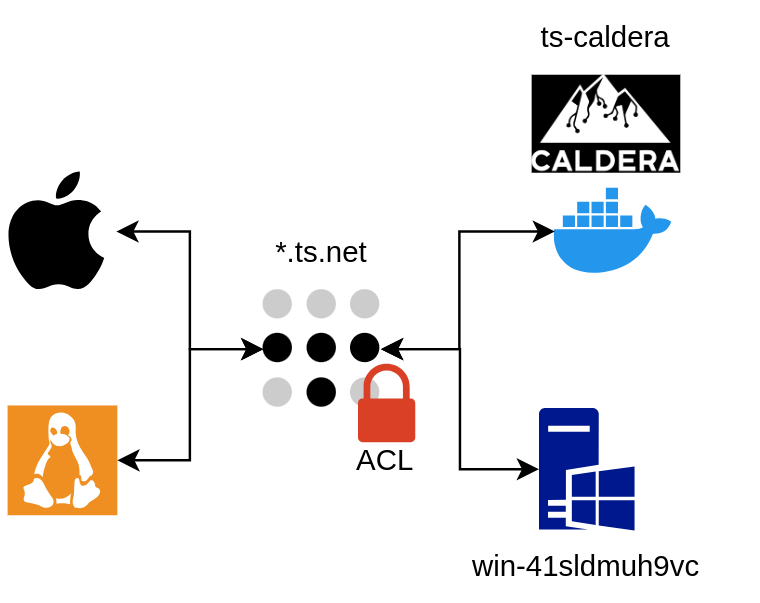
\includegraphics[width=0.5\textwidth]{images/infra_scheme.png}
    \caption{Architecture de l'environnement de travail}
    \label{fig:architecture}
\end{figure}
\subsubsection{Fonctionnalités}

Les principales fonctionnalités de Tailscale incluent :
\begin{itemize}
    \item \textbf{Configuration simplifiée} : Configuration automatisée de l'infrastructure réseau (routage, contrôle des accès, DNS, ...).
    \item \textbf{Sécurité renforcée} : Chiffrement avec Wireguard.
    \item \textbf{Accès à distance} : Permet de se connecter au réseau même à distance.
    \item \textbf{Gestion des identités} : Tailscale utilise des ACL pour contrôler l'accès aux ressources. Il s'intègre avec des systèmes d'authentification tiers comme Google, Microsoft, Okta, etc.
    \item \textbf{Interopérabilité} : Fonctionne sur plusieurs plateformes comme Windows, macOS, Linux, iOS et Android.
\end{itemize}

\subsubsection{Avantages}

Tailscale présente plusieurs avantages tels que :
\begin{itemize}
    \item \textbf{Facilité de prise en main} : Il suffit d'installer le client sur les appareils et de se connecter avec un compte ou une clé.
    \item \textbf{Performance} : Faible latence et faible consommation de ressources grâce à WireGuard.
    \item \textbf{Sécurité} : Chiffrement de bout en bout et gestion fine des autorisations.
\end{itemize}

\subsubsection{Cas d'usage}

Tailscale peut être utilisé dans divers scénarios :
\begin{itemize}
    \item \textbf{Accès sécurisé aux ressources internes} : Par exemple, accéder à des serveurs ou bases de données internes.
    \item \textbf{Collaboration entre équipes distantes} : Permet de travailler ensemble sur un même réseau, une même infrastructure mais à distance
    \item \textbf{Administration système} : Gérer des machines distantes sans exposer les ports au public.
    \item \textbf{Création de réseaux privés temporaires} : Pour des projets ou des tests spécifiques.
\end{itemize}

\newpage
\section{Déroulement du Projet}

L'étude est composée de plusieurs étapes clées : \\
Dans une premier temps, nous allons réaliser une étude préalable pour comprendre et maîtriser les différents outils présentés précedemment.
Ensuite, nous allons émuler plusieurs APT afin d'évaluer l'efficacité de l'outil Caldera dans un premier temps.
Puis, dans un second temps, nous analyserons l'utilité des outils de détection comme Aurora ainsi que les difficultés liées.
Enfin, nous conclurons quant à l'utilité et les forces des outils présentés 

\subsection{Étude préalable}
\subsubsection{Installation des outils}

La première étape de l'étude a consisté à installer les différents outils présentés précédemment.

\bigskip

Pour commencer, nous avons utiliser Tailscale pour créer un réseau virtuel qui nous sert d'environnement de travail.
Ensuite, nous avons instancié Caldera à l'aide de Docker.
Nous avons rencontré ensuite certaines difficultés pour faire fonctionner Caldera dans ce conteneur mais aussi à se connecter à l'interface web depuis une autre machine du réseau Tailscale.
Enfin, nous avons déployer une machine virtuelle Windows serveur 2019 sur laquelle nous avons installé l'EDR Aurora.
Par la suite nous avons configuré un Active Directory (AD) sur cette même machine pour une simulation plus proche d'un environnement d'entreprise.

\subsubsection{Prise en main des outils}
\begin{enumerate}
    \item \textbf{Caldera} : 
    Pour prendre en main l'outil Caldera, il nous a fallu commencer par comprendre comment fonctionne l'émulation d'attaque.
    Ainsi, nous avons utilsés les salles de \textit{TryHackMe} à ce sujet. \\

    Pour cela nous avons dans un premier temps appris le concept d'émulation d'attaque, non seulement d'un point de vue technique mais aussi d'un point vue entreprise (entente avec l'entreprise cible, méthodologie, rapport).
    Dans un second temps, nous avons mis en pratique nos connaissances via l'outil \verb|Invoke-Atomic| développé par le groupe Atomic Red Team pour l'émulation d'APT, de techniques via Powershell. \\

    Enfin nous avons réaliser le cours sur l'outil Caldera qui nous a appris à manier l'outil et ses différentes facettes. 

    \item \textbf{Windows \- Event Manager} :
    Afin de mieux comprendre comment fonctionne les attaques d'un point de vue de la victime et l'EDR Aurora, nous avons décider d'apprendre et de comprendre la gestion des journaux sur Windows.
    Ainsi, nous avons utilisé les outils suivant : \verb|Get-WinEvent|, \verb|wevtutil.exe| ou encore \verb|XPath Queries|.
    Nous avons utilisé la salle TryHackMe associée.
    Cela nous a permis de comprendre la formes des techniques au sein des journaux, ainsi que la manière de les trier et de les analyser. \\
    
    \item \textbf{Aurora EDR} :
    Nous avons ensuite pris en main l'outil Aurora EDR.
    Pour cela, nous avons utilisé la documentation de l'outil qui nous a permis de comprendre comment fonctionne l'outil et comment il s'intègre dans notre environnement.
    Puis, nous avons réaliser la leçon de mise en pratique de TryHackMe. \\
\end{enumerate}

\newpage
\subsection{Premier scénario}
L'objectif de ce premier scénario était de prendre en mains les diverses aspects de Caldera dont les :
\begin{itemize}
    \item Techniques
    \item Adversaires
    \item Opérations
\end{itemize}

Dans ce dernier, nous avions pour objectif de simuler une attaque simple.
Ainsi, nous avons choisi d'effectuer une extraction de données sur le système cible Windows Server.

Pour cela, nous avons créer deux techniques :
\begin{itemize}
    \item \textbf{T1005} : Data from Local System
    \item \textbf{T1003.003} : Exfiltration Over Web Service : Exfiltration to Cloud Storage
\end{itemize}

La première technique utilise l'outil \verb|ntdsutil| pour exfiltrer les données de l'Active Directory.
C'est un outil de ligne de commande qui permet d'interagir avec la base de données Active Directory.
Il est utilisé pour effectuer des opérations de maintenance et de gestion sur les bases de données AD.
Il permet notamment d'extraire la base de données AD, de la sauvegarder ou de la restaurer.

Ainsi, nous allons générer le fichier \verb|ntds.dit| qui contient les informations de l'Active Directory à l'aide de la commande suivante :
\lstinputlisting[caption={Data From Local System}]{../scripts/Get-NTDS.ps1}

On retrouvera donc la base de données de l'Active Directory \verb|ntds.dit| dans le répertoire \verb|C:\Windows\Temp\NTDS\Active Directory\|.
La seconde technique utilise un serveur web externe pour exfiltrer ces données à l'aide d'une requête POST :
\lstinputlisting[caption={Exfiltration Over Web Service}]{../scripts/Push-NTDS.ps1}
Cette commande va permettre d'exfiltrer le fichier \verb|ntds.dit| vers le serveur web externe qui se trouve également sur le Tailnet. \\

Nous avons ensuite créé un adversaire qui va utiliser ces deux techniques dans la partie \textit{Adversaries} de Caldera.
Il s'agit ici de l'adversaire \textbf{APT0}, un adversaire fictif pour ce premier scénario.

\begin{figure}[h!]
    \centering
    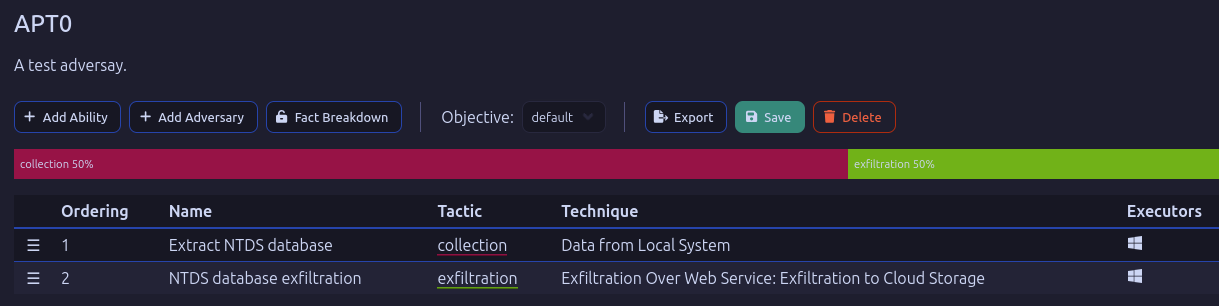
\includegraphics[width=1\textwidth]{images/caldera/apt0_adversary.png}
    \caption{Adversaire APT0}
    \label{fig:apt0_adversary}
\end{figure}

Finalement, nous pouvons lancer une opération et observer le résultat sur Caldera.
On retrouve bien les deux techniques définies précédemment.
On remarque que les deux techniques ont bien été exécutées, sur l'hôte WIN-41SLDMUH9VC et que la sortie de la seconde commande affiche bien un succès.
Ce qui signifie que la base de données a bien été extraite puis exfiltrée vers le serveur web externe.

\begin{figure}[h!]
    \centering
    \begin{subfigure}{0.95\textwidth}
        \centering
        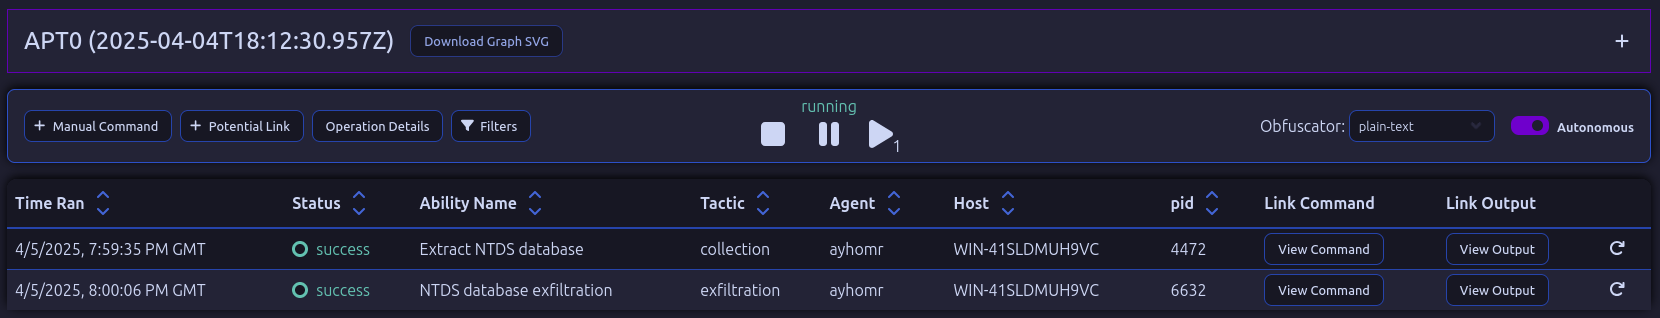
\includegraphics[width=1\textwidth]{images/caldera/apt0_operation.png}
        \caption{Affichage des techniques utilisées}
        \label{fig:apt0_operation_1}
    \end{subfigure}
    \begin{subfigure}{0.3\textwidth}
        \centering
        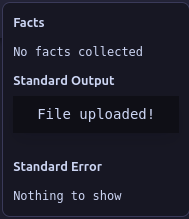
\includegraphics[width=1\textwidth]{images/caldera/apt0_operation_result.png}
        \caption{Résultat de la seconde technique}
        \label{fig:apt0_operation_2}
    \end{subfigure}
    \caption{Opération pour APT0}
\end{figure}

Ainsi, nous avons pu émuler une attaque simple à l'aide de Caldera en utilisant les techniques du cadre MITRE ATT\&CK.

\newpage
\subsection{Second scénario}

Dans ce second scénario, nous allons émuler une attaque plus complexe.
Nous avons choisi d'émuler l'APT \textbf{AKIRA} qui est un rançongiciel.

Voici les techniques utilisées d'après le cadre MITRE ATT\&CK \cite{AkiraGOLDSAHARA} :
\begin{table}[h!]
    \centering
    \begin{tabular}{|l|l|p{10cm}|}
        \hline
        \textbf{Domain} & \textbf{ID} & \textbf{Name and Use} \\ \hline
        Enterprise & T1531 & \textbf{Account Access Removal}: Akira deletes administrator accounts in victim networks prior to encryption. \\ \hline
        Enterprise & T1560.001 & \textbf{Archive Collected Data: Archive via Utility}: Akira uses utilities such as WinRAR to archive data prior to exfiltration. \\ \hline
        Enterprise & T1486 & \textbf{Data Encrypted for Impact}: Akira encrypts files in victim environments as part of ransomware operations. \\ \hline
        Enterprise & T1213.002 & \textbf{Data from Information Repositories: SharePoint}: Akira has accessed and downloaded information stored in SharePoint instances as part of data gathering and exfiltration activity. \\ \hline
        Enterprise & T1482 & \textbf{Domain Trust Discovery}: Akira uses the built-in Nltest utility or tools such as AdFind to enumerate Active Directory trusts in victim environments. \\ \hline
        Enterprise & T1567.002 & \textbf{Exfiltration Over Web Service: Exfiltration to Cloud Storage}: Akira will exfiltrate victim data using applications such as Rclone. \\ \hline
        Enterprise & T1133 & \textbf{External Remote Services}: Akira uses compromised VPN accounts for initial access to victim networks. \\ \hline
        Enterprise & T1657 & \textbf{Financial Theft}: Akira engages in double-extortion ransomware, exfiltrating files then encrypting them, in order to prompt victims to pay a ransom. \\ \hline
        Enterprise & T1219 & \textbf{Remote Access Software}: Akira uses legitimate utilities such as AnyDesk and PuTTy for maintaining remote access to victim environments. \\ \hline
        Enterprise & T1018 & \textbf{Remote System Discovery}: Akira uses software such as Advanced IP Scanner and MASSCAN to identify remote hosts within victim networks. \\ \hline
        Enterprise & T1078 & \textbf{Valid Accounts}: Akira uses valid account information to remotely access victim networks, such as VPN credentials. \\ \hline
    \end{tabular}
    \caption{Techniques utilisées par le rançongiciel Akira}
    \label{tab:akira_techniques}
\end{table}

Nous avons donc créé un adversaire qui utilise ces techniques.
Dans la liste des cacacités proposés par Caldera (provenant d'Atomic Red Team), nous avons choisi d'utiliser les capacités les plus proches des descriptions fournies par MITRE ATT\&CK.
Nous avons donc utilisé les capacités suivantes :

\begin{figure}[h!]
    \centering
    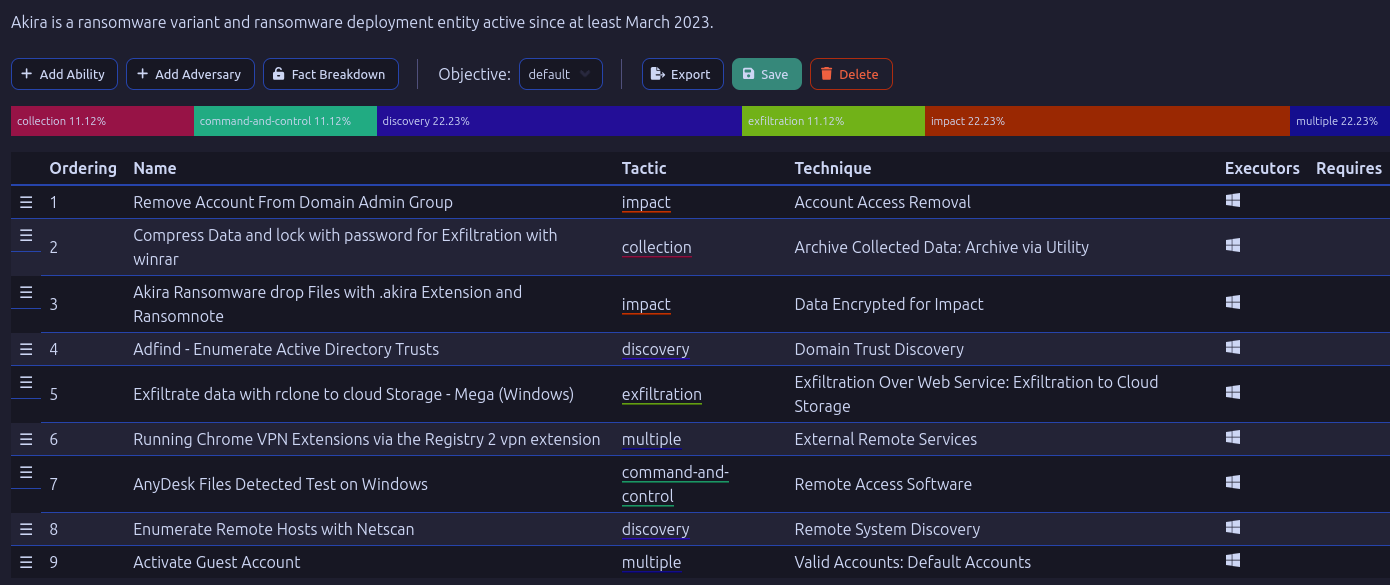
\includegraphics[width=1\textwidth]{images/caldera/akira_adversary.png}
    \caption{Adversaire APT AKIRA}
    \label{fig:akira_adversary}
\end{figure}

Cependant, il a fallu corriger certaines capacités pour qu'elles soient compatibles avec notre environnement. 

\bigskip

Une fois les opérations menées, il reste à analyser les journaux de l'EDR Aurora pour voir si les techniques ont bien été détectées.
Pour cela, il suffit de lancer l'outil Aurora et de se rendre dans l'application Event Viewer de Windows.
Les journaux d'Aurora se trouvent dans le cannal \verb|Application| et la source est \verb|AuroraAgent|.
Dans les captures d'écrans \ref{fig:event_viewer_1} et \ref{fig:event_viewer_2} ci-dessous, un exemple de journal d'Aurora vu dans l'Event Viewer de Windows.

\begin{figure}[h!]
    \centering
    \begin{subfigure}{0.85\textwidth}
        \centering
        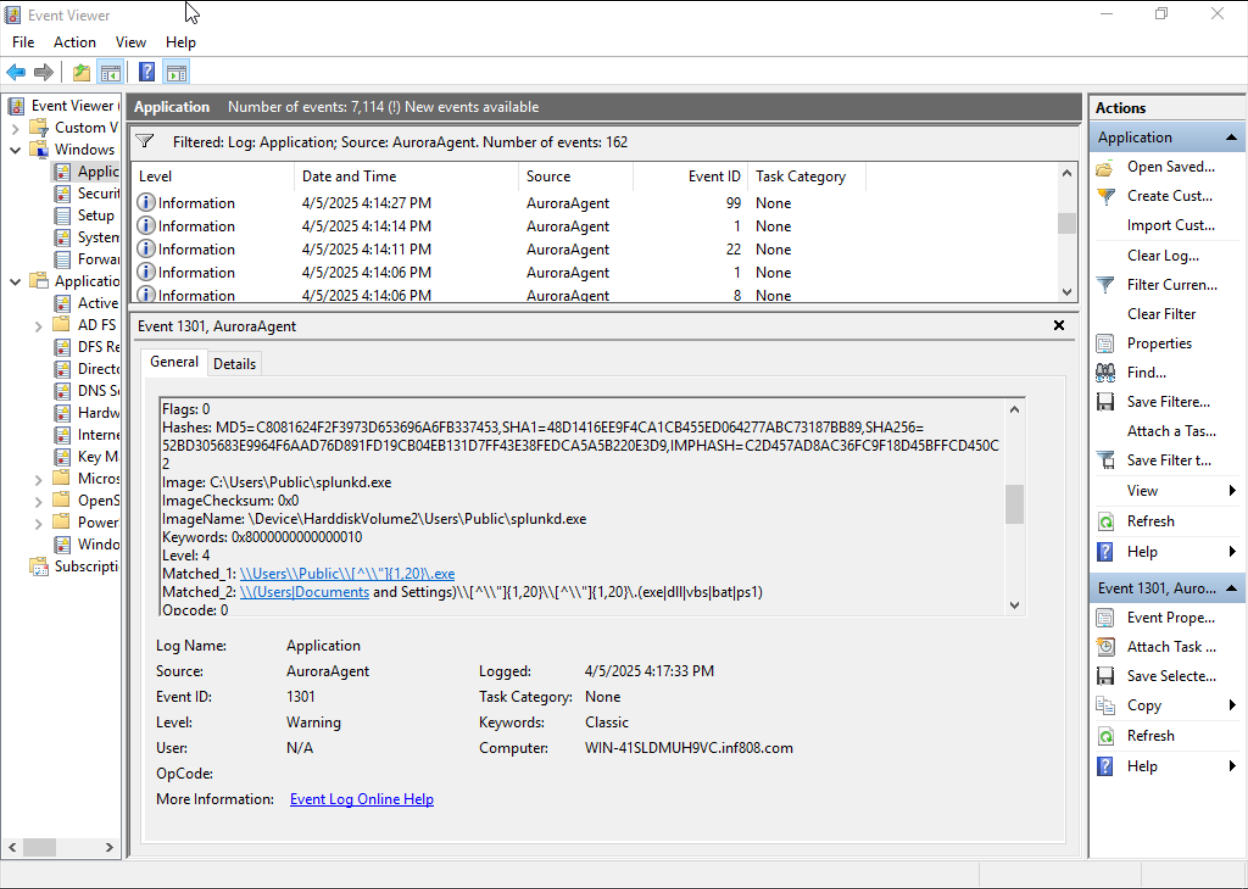
\includegraphics[width=1\textwidth]{images/windows/event_viewer1.png}
        \caption{Première partie du journal}
        \label{fig:event_viewer_1}
    \end{subfigure}
    \begin{subfigure}{0.85\textwidth}
        \centering
        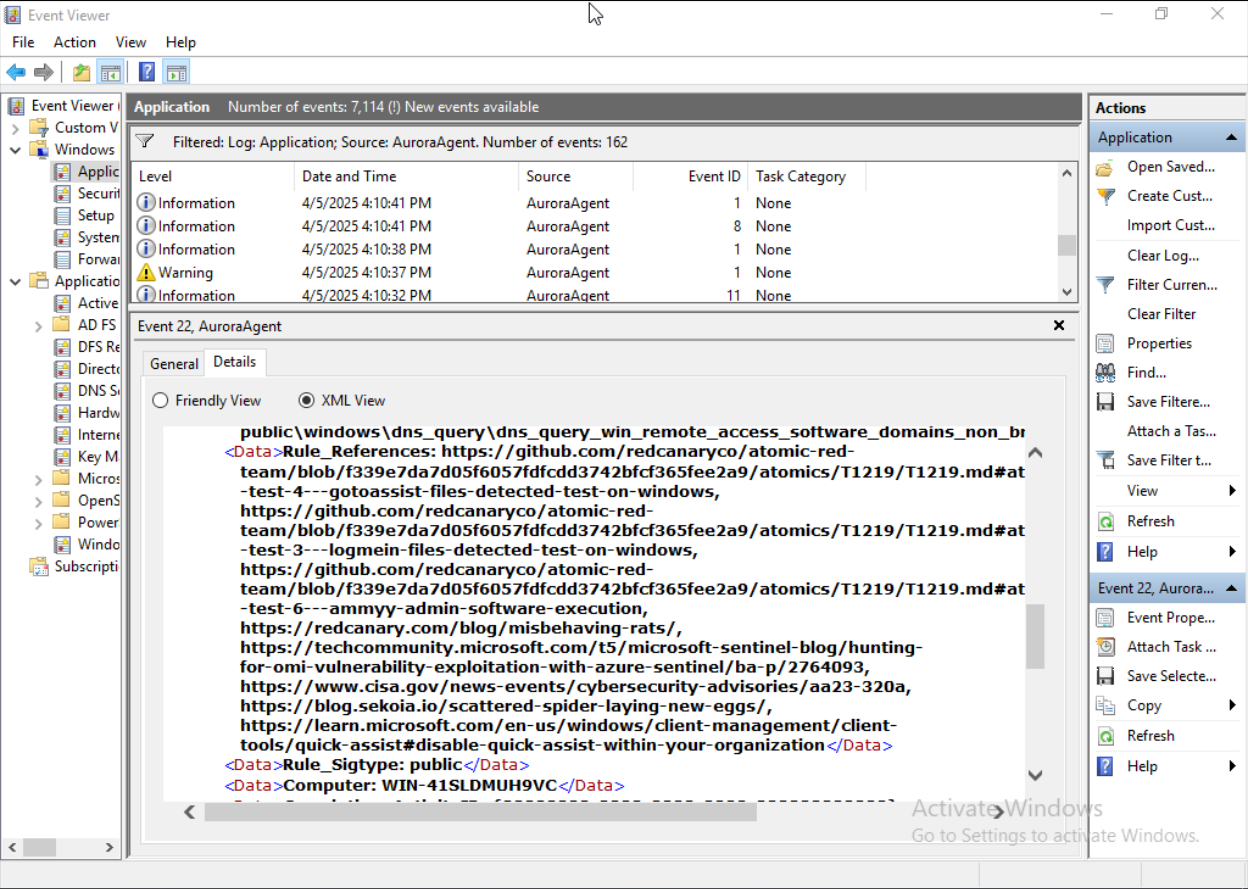
\includegraphics[width=1\textwidth]{images/windows/event_viewer2.png}
        \caption{Seconde partie du journal}
        \label{fig:event_viewer_2}
    \end{subfigure}
    \caption{Event Viewer Windows : journaux d'Aurora}
    \label{fig:event_viewer}
\end{figure}

\bigskip

On remarque donc qu'Aurora a bien détecté l'attaque et mentionne également des techniques utilisées par l'attaquant, ici T1219, dans la partie \textit{Data} de l'onglet détails.
Si l'on regarde dans la liste des techniques de l'attaquant, on remarque que la technique T1219 est bien présente dans la liste des techniques utilisées par l'attaquant.
Il s'agit de la technique \textbf{Remote Access Software} qui correspond à l'utilisation de logiciels de prise de contrôle à distance comme AnyDesk ou PuTTy.

\newpage

À présent, nous avons voulu automatiser la recherche de journaux d'Aurora.
Pour cela, nous avons utilisé le module \verb|Get-WinEvent| de PowerShell.
Celui-ci permet de récupérer les journaux d'événements de Windows.
Il est possible de filtrer pour ne récupérer que les événements d'Aurora.
\begin{itemize}
    \item \textbf{ID} : ID de l'événement
    \item \textbf{TimeCreated} : Date et heure de création de l'événement
    \item \textbf{TTP} : TTP utilisé
    \item \textbf{Level} : Niveau de l'événement selon Aurora
    \item \textbf{CommandLine} : Ligne de commande utilisée
    \item \textbf{ParentCommandLine} : Ligne de commande du processus parent
\end{itemize}

Ci-dessous, l'extrait du premier script qui permet de récupérer les informations suivantes provenants des journaux d'Aurora :

\begin{lstlisting}[caption={Récupération des journaux d'Aurora}, label={lst:aurora_logs}]
$events = Get-WinEvent -LogName "Application" -FilterXPath "*[System[Provider[@Name='AuroraAgent']]]"
\end{lstlisting}

On utilise la commande \verb|Get-WinEvent| avec un filtre XPath pour ne récupérer que les événements d'Aurora.
XPath est un langage de requête qui permet de sélectionner des nœuds dans un document XML, il a été créé par W3C \cite{XMLPathLanguage}.
Ce premier script nous permet d'obtenir les TTP les plus courantes repérées par Aurora.
Dans nos essais, le script a pu travailler sur 1135 événements d'Aurora et a pu extraire 282 TTPs, avec l'ajout de quelques commandes pour filter le résultat on obtient :

\begin{lstlisting}[caption={Recherche des TTP dans les journaux d'Aurora}, label={lst:ttp_logs}]
PS C:\Users\Administrator> .\Get-TTP.ps1 | Group-Object -Property TTP | ForEach-Object {[PSCustomObject]@{
    TTP = $_.Name
    Count = $_.Count
    EventDetail = $_.Group
}} | Sort-Object -Property Count

    TTP       Count EventDetail
    ---       ----- -----------
    T1027.004     1 {@{TPP=T1027.004;...
    T1047         1 {@{TPP=T1047;...
    T1562.004     2 {@{TPP=T1562.004;...
    T1059.001     2 {@{TPP=T1059.001;...
    T1053.005     7 {@{TPP=T1053.005;...
    T1560.001    18 {@{TPP=T1560.001;...
    T1087.002    27 {@{TPP=T1087.002;...
    T1219       224 {@{TPP=T1219;...
\end{lstlisting}

On obtient un tableau avec les TTPs, le nombre d'occurrences et les détails des événements liés au TTP.
On peut donc avoir tous les événements liés à un TTP en particulier.
On remarque aussi que la technique T1219 est la plus courante dans les journaux d'Aurora.
Ainsi, il est possible de récupérer certaines TTPs émulées par Caldera.

\bigskip

Ensuite, nous avons voulu savoir si ces TTPs étaient utilisées par des APTs.
Pour cela, nous avons utilisé le second script \verb|Match-TTP-APT.ps1| qui permet de comparer les TTPs extraites avec la base de données MITRE ATT\&CK.
La combinaison des deux scripts nous permet d'obtenir une liste d'APT qui seraient susceptibles d'utiliser les TTP repérées par Aurora.
\begin{lstlisting}[caption={Identification des APTs}, label={lst:apt_logs}]
PS C:\Users\Administrator> .\Get-TTP.ps1 | Group-Object -Property TPP | ForEach-Object {[PSCustomObject]@{
    TTP = $_.Name
    Count = $_.Count
    EventDetail = $_.Group
}} | Sort-Object -Property Count | .\Match-TTP-APT.ps1

    [+] Analyse des TTP extraits avec MITRE ATT&CK...
    [*] Téléchargement de la base ATT&CK...

    ==== TOP GROUPES IDENTIFIÉS ====

    GroupName     MatchCount MatchingTTPs
    ---------     ---------- ------------
    MuddyWater             7 T1027.004, T1047, T1053.005, T1059.001, T1087.002, T1219, T1560.001
    ToddyCat               6 T1047, T1053.005, T1059.001, T1087.002, T1560.001, T1562.004
    FIN13                  5 T1047, T1053.005, T1059.001, T1087.002, T1560.001
    Mustang Panda          5 T1047, T1053.005, T1059.001, T1219, T1560.001
    menuPass               5 T1047, T1053.005, T1059.001, T1087.002, T1560.001
    Wizard Spider          5 T1047, T1053.005, T1059.001, T1087.002, T1560.001
    Magic Hound            5 T1047, T1053.005, T1059.001, T1560.001, T1562.004
    Kimsuky                5 T1053.005, T1059.001, T1219, T1560.001, T1562.004
    Chimera                5 T1047, T1053.005, T1059.001, T1087.002, T1560.001
    APT41                  5 T1047, T1053.005, T1059.001, T1087.002, T1560.001
\end{lstlisting}

Au final, on obtient une liste d'APT qui utilisent les TTPs repérées par Aurora.
L'APT Akira ne fait pas partie de la liste.

\section{Observation}

APT trouvées correspondent pas à AKIRA
=> Tous les TTPs ne sont pas forcément détectés par Aurora
=> méthode pas forcément fiable

\section{Conclusion}



\newpage
\section{Listings}
\lstinputlisting[caption={Exfiltration Over Web Service}, label={get-ttp}]{../scripts/Get-TTP.ps1}

\lstinputlisting[caption={Exfiltration Over Web Service}, label={match-ttp}]{../scripts/Match-TTP-APT.ps1}

\newpage
\bibliographystyle{unsrtnat} % or any other style like apalike, alpha, etc.
\bibliography{bib/main}

\end{document}

